% file: chap1.tex

\chapter{使用神经网络识别手写数字}
\label{ch:UsingNeuralNetsToRecognizeHandwrittenDigits}

人类视觉系统是世界上众多奇迹之一。看看下面的手写数字序列:
\begin{center}
  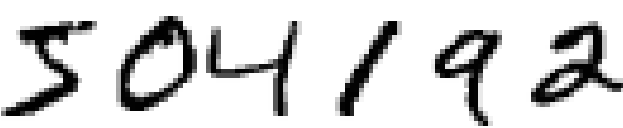
\includegraphics[width=64pt]{digits}\label{fig:digits}
\end{center}

大多数人毫不费力就能够认出这些数字为504192。这么容易反而让人觉着迷惑了。在人类的
每个脑半球中,有着一个初级视觉皮层,常称为V1,包含1亿4千万个神经元及数百亿条神经
元间的连接。但是人类视觉不是就只有V1,还包括整个视觉皮层 —— V2、V3、V4和V5 —— 他
们逐步地进行更加复杂的图像处理。人类的头脑就是一台超级计算机,通过数十亿年的进化
不断地演变,最终能够极好地适应理解视觉世界的任务。识别手写数字也不是一件简单的事。
尽管人类在理解我们眼睛展示出来的信息上非常擅长,但几乎所有的过程都是无意识地。所
以,我们通常并不能体会自身视觉系统解决问题的困难。

如果你尝试写出计算机程序来识别诸如上面的数字,就会明显感受到视觉模式识别的困难。
看起来人类一下子就能完成的任务变得特别困难。关于我们识别形状 —— ``9顶上有一个圈,
右下方则是一条竖线''这样的简单直觉 —— 实际上算法上就很难轻易表达出来了。而在你试
着让这些识别规则越发精准时,就会很快陷入各种混乱的异常或者特殊情形的困境中。看起
来毫无希望。

神经网络以另一种方式看待这个问题。其主要思想是获取大量的手写数字,常称作训练样本,
\begin{center}
  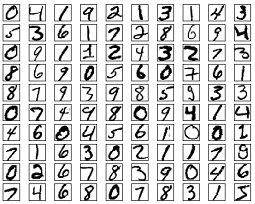
\includegraphics[width=200pt]{mnist_100_digits}
\end{center}

然后开发出一个可以从这些训练样本中进行学习的系统。换言之,神经网络使用样本来自动
推断出识别手写数字的规则。另外,通过增加训练样本的数量,网络可以学到更多关于手写
数字的知识,这样就能够提升自身的准确性。所以,上面例子中我们只是展出了 100 个训
练数字样本,而通过使用数千或者数百万或者数十亿的训练样本我们也许能够得到更好的手
写数字识别器。

本章我们将实现一个可以识别手写数字的神经网络。这个程序仅仅 74 行,不适用特别的神
经网络库。然而,这个短小的网络不需要人类帮助便可以超过 96\% 的准确率识别数字。而
且,在后面的章节,我们会发展出将准确率提升到 99\% 的技术。实际上,最优的商业神经
网络已经足够好到被银行和邮局分别用在账单核查和识别地址上了。

手写识别常常被当成学习神经网络的原型问题,因此我们聚焦在这个问题上。作为一个原型,
它具备一个关键点:挑战性 —— 识别手写数字并不轻松 —— 但也不会难到需要超级复杂的解
决方法,或者超大规模的计算资源。另外,这其实也是一种发展出诸如深度学习更加高级的
技术的方法。所以,整本书我们都会持续地讨论手写数字识别问题。本书后面部分,我们会
讨论这些想法如何用在其他计算机视觉的问题或者语音、自然语言处理和其他一些领域中。

当然,如果仅仅为了编写一个计算机程序来识别手写数字,本章的内容可以简短很多!但前
进的道路上,我们将扩展出很多关于神经网络的关键的思想,其中包括两个重要的人工神经
元(感知器和S型神经元),以及标准的神经网络学习算法,即随机梯度下降算法。自始至
终,我专注于解释事情的原委,并构筑你对神经网络的直观感受。这需要一个漫长的讨论,
而不是仅仅介绍些基本的技巧,但这对于更深入的理解是值得的。作为收益,在本章的最后,
我们会准备好了解什么是深度学习,以及它为什么很重要。

\section{感知器}
\label{sec:Perceptrons}

什么是神经网络?一开始,我将解释一种被称为``感知器''的人工神经元。感知器在20世纪
五、六十年代由科学家 \href{http://en.wikipedia.org/wiki/Frank_Rosenblatt}{Frank
  Rosenblatt}
\href{http://books.google.ca/books/about/Principles_of_neurodynamics.html?id=7FhRAAAAMAAJ}{
  发明},其受到 \href{http://en.wikipedia.org/wiki/Warren_McCulloch}{Warren
  McCulloch} 和 \href{http://en.wikipedia.org/wiki/Walter_Pitts}{Walter Pitts} 早
期的\href{http://scholar.google.ca/scholar?cluster=4035975255085082870}{工作}的影
响。今天,使用其它人工神经元模型更为普遍 —— 在这本书中,以及更多现代的神经网络工
作中,主要使用的是一种叫做 S 型神经元\footnote{译注:英文为``Sigmoid Neutrons'',
  有些神经网络的中文翻译中直接使用英文,其实这里 -oid 词根是指``\ldots 似的'', 结
  合下文会提到的 $\sigma$ (小写的希腊字母 sigma)\hyperref[fig:sigmoid_graph]{曲
    线}形状,本书中统一翻译为 S 型神经元。}的神经元模型。我们很快会讲到S型神经元。
但是要理解为什么S型神经元被定义为那样的方式,值得花点时间先来理解下感知器。

感知器是如何工作的呢?一个感知器接受几个二进制输入,$x_1,x_2,\ldots$,并产生一个二
进制输出:
% tikz0.png
\begin{center}
  \begin{tikzpicture}
    [inner sep=0pt,minimum size=10mm]
    \node (perceptron) at (0, 0) [circle,draw] {};
    \node (output) at (2.25, 0) {\;output};
    \node (x1) at (-2.25, 1) {$x_1$};
    \node (x2) at (-2.25, 0) {$x_2$};
    \node (x3) at (-2.25, -1) {$x_3$};
    \draw [->] (x1) to (perceptron);
    \draw [->] (x2) to (perceptron);
    \draw [->] (x3) to (perceptron);
    \draw [->] (perceptron) to (output);
  \end{tikzpicture}
\end{center}

示例中的感知器有三个输入,$x_1,x_2,x_3$。通常可以有更多或更少输入。Rosenblatt 提
议一个简单的规则来计算输出。他引入\emph{权重},$w_1,w_2,\ldots$,表示相应输入对
于输出重要性的实数。神经元的输出,$0$或者$1$,则由分配权重后的总和$\sum_j w_j
x_j$小于或者大于一些\emph{阈值}决定。和权重一样,阈值是一个实数,一个神经元的参
数。用更精确的代数形式:
\begin{equation}
  \text{output} = \begin{cases}
    0 & \quad \text{if } \sum_j w_j x_j \leq \text{ threshold} \\
    1 & \quad \text{if } \sum_j w_j x_j > \text{ threshold} \\
  \end{cases}
  \tag{1}
\end{equation}

这就是一个感知器所要做的所有事情!

这是基本的数学模型。你可以将感知器看作依据权重来作出决定的设备。让我举个例子。这
不是非常真实的例子,但是容易理解,而且很快我们会有根多实际的例子。假设这个周末就
要来了,你听说你所在的城市有个奶酪节。你喜欢奶酪,正试着决定是否去参加。你也许会
通过给三个因素设置权重来作出决定:
\begin{enumerate}
\item 天气好吗?
\item 你的男朋友或者女朋友会不会陪你去?
\item 这个节日举办的地点是否靠近交通站点?(你没有车)
\end{enumerate}

你可以把这三个因素对应地用二进制变量$x_1,x_2$和$x_3$来表示。例如,如果天气好,我
们把$x_1 = 1$,如果不好,$x_1 = 0$。类似地,如果你的男朋友或女朋友同去,$x_2 =
1$,否则$x_2 = 0$。$x_3$也类似地表示交通情况。

现在,假设你是个嗜好奶酪的吃货,以至于即使你的男朋友或女朋友不感兴趣,也不管路有
多难走都乐意去。但是也许你确实厌恶糟糕的天气,而且如果天气太糟你也没法出门。你可
以使用感知器来给这种决策建立数学模型。一种方式是给天气权重选择为 $w_1 = 6$ ,其
它条件为 $w_2 = 2$ 和 $w_3 = 2$。$w_1$ 被赋予更大的值,表示天气对你很重要,比你
的男朋友或女朋友陪你,或者最近的交通站重要的多。最后,假设你将感知器的阈值设为
$5$。这样,感知器实现了期望的决策模型,只要天气好就输出 $1$,天气不好则为 $0$。
对于你的男朋友或女朋友是否想去,或者附近是否有公共交通站,其输出则没有差别。

随着权重和阈值的变化,你可以得到不同的决策模型。例如,假设我们把阈值改为 $3$ 。
那么感知器会按照天气好坏,或者结合交通情况和你男朋友或女朋友同行的意愿,来得出结
果。换句话说,它变成了另一个不同的决策模型。降低阈值则表示你更愿意去。

很明显,感知器不是人做出决策使用的全部模型。但是这个例子说明了一个感知器如何能权
衡不同的依据来决策。这看上去也可以大致解释一个感知器网络能够做出微妙的决定:
% tikz1.png
\begin{center}
  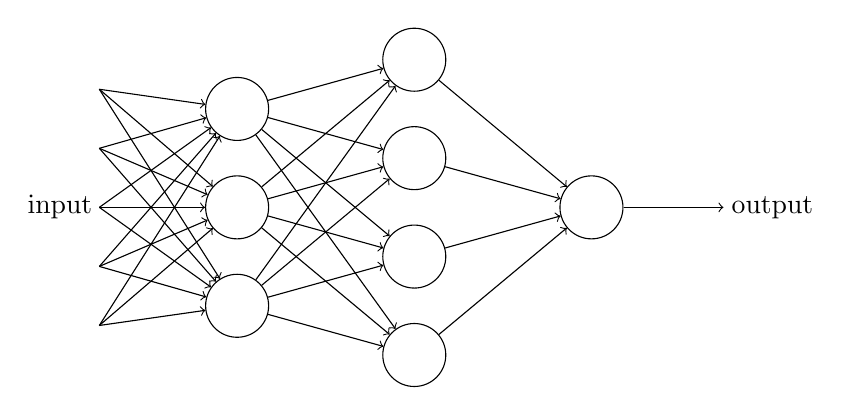
\begin{tikzpicture}
    [inner sep=0pt,minimum size=8mm]

    % input label:
    \node (input) at (-4.5, 0) {input};

    % leftmost perceptrons:
    \node (pl1) at (-2.25, 1.25) [circle,draw] {};
    \node (pl2) at (-2.25, 0) [circle,draw] {};
    \node (pl3) at (-2.25, -1.25) [circle,draw] {};

    % middle perceptrons:
    \node (pm1) at (0, 1.875) [circle,draw] {};
    \node (pm2) at (0, 0.625) [circle,draw] {};
    \node (pm3) at (0, -0.625) [circle,draw] {};
    \node (pm4) at (0, -1.875) [circle,draw] {};

    % rightmost perceptron:
    \node (pr) at (2.25, 0) [circle,draw] {};

    % output:
    \node (output) at (4.5, 0) {\;output};

    % connect nodes:

    \draw [->] (-4, 1.5) to (pl1);
    \draw [->] (-4, 1.5) to (pl2);
    \draw [->] (-4, 1.5) to (pl3);

    \draw [->] (-4, 0.75) to (pl1);
    \draw [->] (-4, 0.75) to (pl2);
    \draw [->] (-4, 0.75) to (pl3);

    \draw [->] (-4, 0) to (pl1);
    \draw [->] (-4, 0) to (pl2);
    \draw [->] (-4, 0) to (pl3);

    \draw [->] (-4, -0.75) to (pl1);
    \draw [->] (-4, -0.75) to (pl2);
    \draw [->] (-4, -0.75) to (pl3);

    \draw [->] (-4, -1.5) to (pl1);
    \draw [->] (-4, -1.5) to (pl2);
    \draw [->] (-4, -1.5) to (pl3);

    \draw [->] (pl1) to (pm1);
    \draw [->] (pl1) to (pm2);
    \draw [->] (pl1) to (pm3);
    \draw [->] (pl1) to (pm4);
    \draw [->] (pl2) to (pm1);
    \draw [->] (pl2) to (pm2);
    \draw [->] (pl2) to (pm3);
    \draw [->] (pl2) to (pm4);
    \draw [->] (pl3) to (pm1);
    \draw [->] (pl3) to (pm2);
    \draw [->] (pl3) to (pm3);
    \draw [->] (pl3) to (pm4);
    \draw [->] (pm1) to (pr);
    \draw [->] (pm2) to (pr);
    \draw [->] (pm3) to (pr);
    \draw [->] (pm4) to (pr);
    \draw [->] (pr) to (output);

  \end{tikzpicture}
\end{center}

在这个网络中,第一列感知器 —— 我们称其为第一层感知器 —— 通过权衡输入证据做出三个
非常简单的决定。那第二层的感知器呢?每一个都在权衡第一层的决策结果并做出决定。以
这种方式,一个第二层中的感知器可以比第一层中的做出更复杂和抽象的决策。在第三层中
的感知器甚至能进行更复杂的决策。以这种方式,一个多层的感知器网络可以从事复杂巧妙
的决策。

顺便提一下,当我定义感知器时我说的是感知器只有一个输出。在上面的网络中感知器看上
去像是有多个输出。实际上,他们仍然是单输出的。多个感知器输出箭头仅仅便于说明一个
感知器的输出被用于其它感知器的输入。它和把单个输出线条分叉相比,显得讨巧些。

让我们简化感知器的数学描述。条件 $\sum_j w_j x_j$ 看上去有些冗长,我们可以创建两
个符号的变动来简化。第一个变动是把 $\sum_j w_j x_j$ 改写成点乘,$w \cdot x
\equiv \sum_j w_j x_j$,这里 $w$ 和 $x$ 对应权重和输入的向量。第二个变动是把阈值
移到不等式的另一边,并用感知器的偏差 $b \equiv -threshold$ 代替。用偏差而
不是阈值,那么感知器的规则可以重写为:
\begin{equation}
  \text{output} = \begin{cases}
    0 & \quad \text{if } w\cdot x + b \leq 0 \\
    1 & \quad \text{if } w\cdot x + b > 0
  \end{cases}
  \tag{2}
\end{equation}

我们可以把偏差看作一种表示让感知器输出 $1$(或者用生物学的术语,即激活感知器)有
多容易的估算。对于具有一个非常大偏差的感知器来说,输出 $1$ 是很容易的。但是如果偏
差是一个非常大的负数,输出 $1$ 则很困难。很明显,引入偏差只是我们描述感知器的一个
很小的变动,但是我们后面会看到它引导更进一步的符号简化。因此,在这本书的后续部分,
我们不再用阈值,而总是使用偏差。

我已经描述过感知器是一种权衡证据来做出决策的方法。感知器被采用的另一种方式,是计
算基本的逻辑功能,即我们通常认为的基础,例
如``\emph{与}'',``\emph{或}''和``\emph{与非}''。例如,假设我们有个两个输入的感知
器,每个权重为 $-2$,总偏差为$3$。这是我们的感知器:
% tikz2.png
\begin{center}
  \begin{tikzpicture}
    [inner sep=0pt,minimum size=12mm]
    \node (perceptron) at (0, 0) [circle,draw] {$3$};
    \node (output) at (2.65, 0) {};
    \node (x1) at (-2.65, 1) {$x_1$};
    \node (x2) at (-2.65, -1) {$x_2$};
    \draw [->] (x1) to node [above=-3mm] {$-2$} (perceptron);
    \draw [->] (x2) to node [above=-3mm] {$-2$} (perceptron);
    \draw [->] (perceptron) to (output);
  \end{tikzpicture}
\end{center}

这样我们得到:输入 $00$ 产生输出 $1$,即 $(-2)*0 + (-2)*0 + 3 = 3$ 是正数。这里
我们用 ``$*$'' 来显式地表示乘法。但是输入 $11$ 产生输出 $0$,即 $(-2)*1 + (-2)*1
+ 3 = -1$ 是负数。如此我们的感知器实现了一个与非门!

与非门的例子显示了我们可以用感知器来计算简单的逻辑功能。实际上,我们完全能用感知
器网络来计算任何逻辑功能。原因是与非门是通用运算,那样,我们能在多个与非门之上构
建出任何运算。例如,我们能用与非门构建一个电路,它把两个二进制数 $x_1$ 和 $x_2$
相加。这需要计算按位求和,$x_1 \oplus x_2$,同时当 $x_1$ 和 $x_2$ 都为 $1$ 时进
位设为 $1$,即进位位正好是按位乘积 $x_1x_2$:
% tikz3
\begin{center}
  \begin{tikzpicture}[circuit logic US, large circuit symbols,
    contact/.style={circle, fill=black, minimum size=4pt, inner sep=0pt}]

    \matrix [column sep=1cm,row sep=2mm] {
                                 & \node [nand gate] (n1) {}; &                               \\
      \node [nand gate] (n2) {}; &                            & \node [nand gate] (sum) {};   \\
                                 & \node [nand gate] (n3) {}; &                               \\
                                 &                            & \node [nand gate] (carry) {}; \\
    };

    \node (x1) [left=of n2,yshift=8mm] {$x_1$};
    \node (x2) [left=of n2,yshift=-8mm] {$x_2$};
    \node (text1) [right=of sum] {sum: $x_1 \oplus x_2$};
    \node (text2) [right=of carry] {carry bit: $x_1x_2$};

    % connections:
    \draw (x1.east) -- ++(right:5mm) node [contact] (x1split) {} |- (n1.input 1);
    \draw (x1split) |- (n2.input 1);

    \draw (x2.east) -- ++(right:5mm) node [contact] (x2split) {} |- (n2.input 2);
    \draw (x2split) |- (n3.input 2);

    \draw (n2.output) -- ++(right:5mm) node [contact] (split1) [] {} |- (n1.input 2);
    \draw (split1 |- n3.input 1) node[contact] (split2) {} -- (n3.input 1);
    \draw (split2 |- carry.input 1) node[contact] (split3) {} -- (carry.input 1);

    \draw (split1) -- (split2) -- (split3) |- (carry.input 2);

    \draw (n1.output) -- ++(right:5mm) |- (sum.input 1);
    \draw (n3.output) -- ++(right:5mm) |- (sum.input 2);

    \draw (sum.output) -- (text1.west);
    \draw (carry.output) -- (text2.west);

  \end{tikzpicture}
\end{center}

为了得到相等的感知器网络,我们把所有与非门替换为感知器,其具有两个输入、每个权重
设为 $-2$,总偏差为 $3$。结果我们得到这样的网络。注意我已经把右下的与非门移动了
一点,只是为了在图上更方面画箭头:
% tikz4.png
\begin{center}
  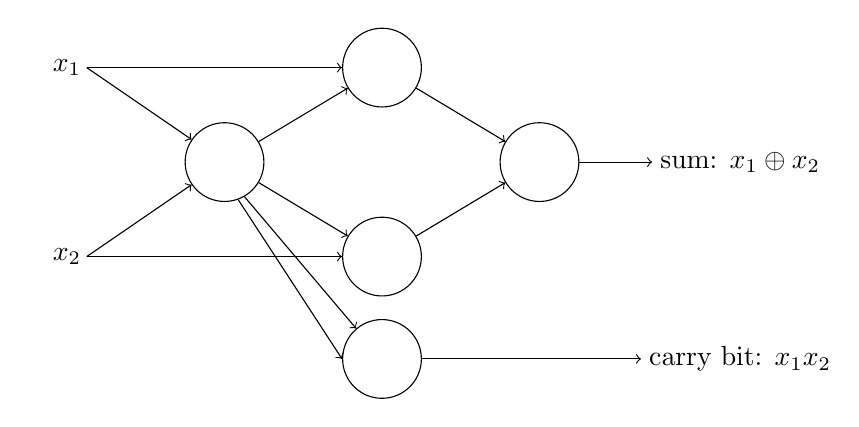
\begin{tikzpicture}
    [inner sep=0pt,minimum size=10mm]
    \node (x1) at (-6, 1.2) {$x_1$};
    \node (x2) at (-6, -1.2) {$x_2$};
    \node (pl1) at (-4, 0) [circle,draw] {};
    \node (pm1) at (-2, 1.2) [circle,draw] {};
    \node (pm2) at (-2, -1.2) [circle,draw] {};
    \node (pm3) at (-2, -2.5) [circle,draw] {};
    \node (pr1) at (0, 0) [circle,draw] {};
    \node (sum) at (2.5, 0) {\;sum: $x_1 \oplus x_2$};
    \node (carrybit) at (2.5, -2.5) {\;carry bit: $x_1x_2$};
    \draw [->] (-5.75, 1.2) to (pl1);
    \draw [->] (-5.75, -1.2) to (pl1);
    \draw [->] (-5.75, 1.2) to (pm1);
    \draw [->] (-5.75, -1.2) to (pm2);
    \draw [->] (pl1) to (pm1);
    \draw [->] (pl1) to (pm2);
    \draw [->] (pl1.-60) to (pm3);
    \draw [->] (pl1.-70) to (pm3.180);
    \draw [->] (pm1) to (pr1);
    \draw [->] (pm2) to (pr1);
    \draw [->] (pr1) to (sum);
    \draw [->] (pm3) to (carrybit);
  \end{tikzpicture}
\end{center}

这个感知器网络中有一个部分值得注意,最左边的感知器的输出被两次作为底部感知器的输
入。当我定义感知器模型时,我没有说过是否允许这种双输出到同一个地方。实际上这不重
要。如果我们不想允许这种形式,那可以简单把两条线合并为到一个权重为 $-4$ 的连接,
而不是两个权重为 $-2$ 的连接。(如果你还没明白,应该停下来证明这是相等的。)随着
这一改变,原先的网络看起来下面描绘的,所有未标记的权重等于 $-2$,所有偏差等于
$3$,标记的单个权重为 $-4$:
% tikz5.png
\begin{center}
  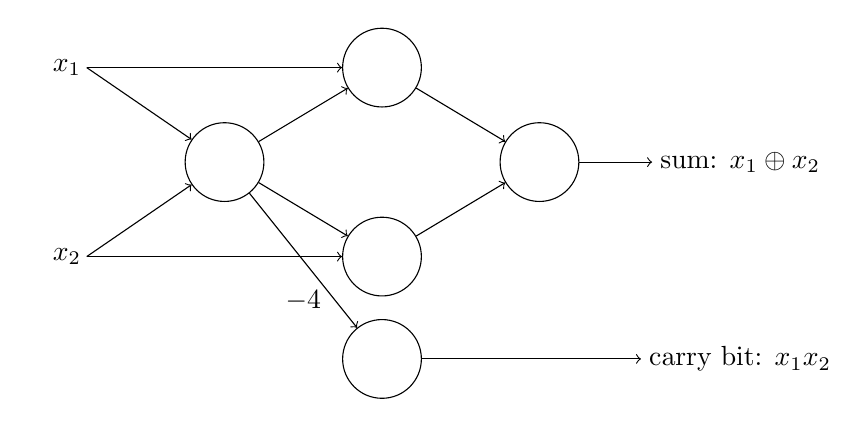
\begin{tikzpicture}
    [inner sep=0pt,minimum size=10mm]
    \node (x1) at (-6, 1.2) {$x_1$};
    \node (x2) at (-6, -1.2) {$x_2$};
    \node (pl1) at (-4, 0) [circle,draw] {};
    \node (pm1) at (-2, 1.2) [circle,draw] {};
    \node (pm2) at (-2, -1.2) [circle,draw] {};
    \node (pm3) at (-2, -2.5) [circle,draw] {};
    \node (pr1) at (0, 0) [circle,draw] {};
    \node (sum) at (2.5, 0) {\;sum: $x_1 \oplus x_2$};
    \node (carrybit) at (2.5, -2.5) {\;carry bit: $x_1x_2$};
    \draw [->] (-5.75, 1.2) to (pl1);
    \draw [->] (-5.75, -1.2) to (pl1);
    \draw [->] (-5.75, 1.2) to (pm1);
    \draw [->] (-5.75, -1.2) to (pm2);
    \draw [->] (pl1) to (pm1);
    \draw [->] (pl1) to (pm2);
    \draw [->] (pl1) to node [below] {$-4$} (pm3);
    \draw [->] (pm1) to (pr1);
    \draw [->] (pm2) to (pr1);
    \draw [->] (pr1) to (sum);
    \draw [->] (pm3) to (carrybit);
  \end{tikzpicture}
\end{center}

目前为止我把像 $x_1$ 和 $x_2$ 这样的输入画成感知器网络左边浮动的变量。实际上,可
以画一层额外的感知器 —— 输入层 —— 来方便对输入编码:
% tikz6.png
\begin{center}
  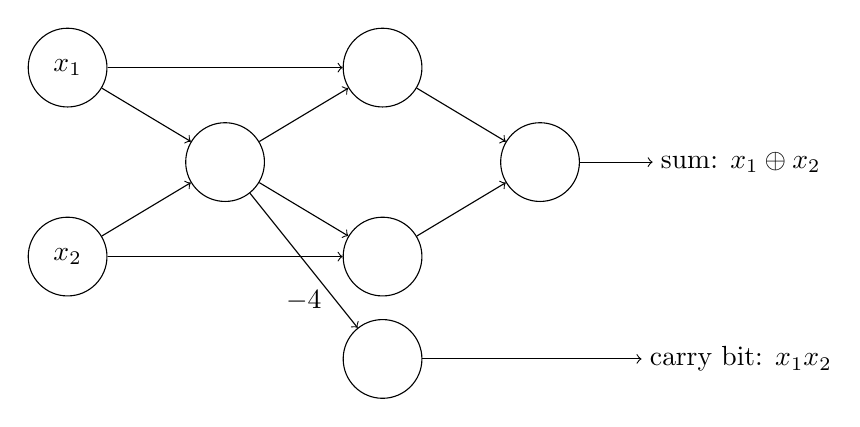
\begin{tikzpicture}
    [inner sep=0pt,minimum size=10mm]
    \node (x1) at (-6, 1.2) [circle,draw] {$x_1$};
    \node (x2) at (-6, -1.2) [circle,draw] {$x_2$};
    \node (pl1) at (-4, 0) [circle,draw] {};
    \node (pm1) at (-2, 1.2) [circle,draw] {};
    \node (pm2) at (-2, -1.2) [circle,draw] {};
    \node (pm3) at (-2, -2.5) [circle,draw] {};
    \node (pr1) at (0, 0) [circle,draw] {};
    \node (sum) at (2.5, 0) {\;sum: $x_1 \oplus x_2$};
    \node (carrybit) at (2.5, -2.5) {\;carry bit: $x_1x_2$};
    \draw [->] (x1) to (pl1);
    \draw [->] (x2) to (pl1);
    \draw [->] (x1) to (pm1);
    \draw [->] (x2) to (pm2);
    \draw [->] (pl1) to (pm1);
    \draw [->] (pl1) to (pm2);
    \draw [->] (pl1) to node [below] {$-4$} (pm3);
    \draw [->] (pm1) to (pr1);
    \draw [->] (pm2) to (pr1);
    \draw [->] (pr1) to (sum);
    \draw [->] (pm3) to (carrybit);
  \end{tikzpicture}
\end{center}

这种对有一个输出但没有输入的感知器的标记法,
% tikz7.png
\begin{center}
  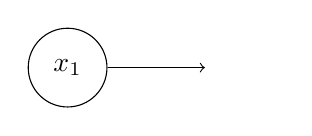
\begin{tikzpicture}
    [inner sep=0pt,minimum size=10mm]
    \node (perceptron) at (0, 0) [circle,draw] {$x_1$};
    \node (output) at (2.25, 0) {};
    \draw [->] (perceptron) to (output);
  \end{tikzpicture}
\end{center}
是一种标准。它并不实际表示一个感知器没有输入。为了看清它,假设我们确实有一个没有
输入的感知器。那么加权和 $\sum_j w_j x_j$ 会总是为零,并且感知器在 $b > 0$ 时输
出 $1$,当 $b \leq 0$时输出 $0$。那样,感知器会简单输出一个固定值,而不是期望值
(上例中的 $x_1$)。倒不如完全不把输入感知器看作感知器,而是简单定义为输出期望值
的特殊单元,$x_1, x_2,\ldots$。

这个加法器的例子演示了一个感知器网络如何用于模拟包含很多与非门的电路。因为与非门
在计算机运算中的通用性,由此可以得出感知器也同样适用的结论。

感知器运算的通用性既是令人鼓舞的,又是令人失望的。令人鼓舞是因为它告诉我们感知器
网络能和其它计算设备一样强大。但是它也令人失望,因为它看上去只不过是一种新的与非
门。这简直不算个大新闻!

然而,实际情况比这一观点认为的更好。其结果是我们可以设计\emph{学习算法},能够自
动调整人工神经元的权重和偏差。这种调整可以响应外部的刺激,而不需要一个程序员的直
接干预。这些学习算法是我们能够以一种根本区别于传统逻辑门的方式使用人工神经元。有
别于显式地设计\emph{与非}或其它门,我们的神经网络能简单地学会解决问题,这些问题
有时候直接用传统的电路设计是很难解决的。

\section{S型神经元}

学习算法听上去非常棒。但是我们怎样给一个神经网络设计这样的算法呢?假设我们有一个
感知器网络,想要用它来解决一些问题。例如,网络的输入可以是一幅手写数字的扫描图像。
我们想要网络能学习权重和偏差,这样网络的输出能正确分类这些数字。为了看清学习是怎
样工作的,假设我们把网络中的权重(或者偏差)做些微小的改动。就像我们马上会看到的,
这一属性会让学习变得可能。这里简要示意我们想要的(很明显这个网络对于手写识别还是
  太简单了!):
% tikz8.png
\begin{center}
  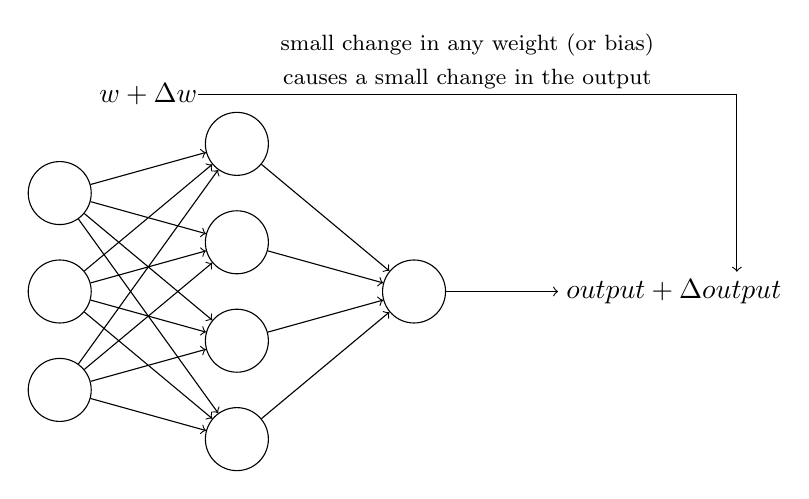
\begin{tikzpicture}
    [inner sep=0pt,minimum size=8mm]

    % leftmost perceptrons:
    \node (pl1) at (-2.25, 1.25) [circle,draw] {};
    \node (pl2) at (-2.25, 0) [circle,draw] {};
    \node (pl3) at (-2.25, -1.25) [circle,draw] {};

    % middle perceptrons:
    \node (pm1) at (0, 1.875) [circle,draw] {};
    \node (pm2) at (0, 0.625) [circle,draw] {};
    \node (pm3) at (0, -0.625) [circle,draw] {};
    \node (pm4) at (0, -1.875) [circle,draw] {};

    % rightmost perceptron:
    \node (pr) at (2.25, 0) [circle,draw] {};

    % output:
    \node (output) at (5.5, 0) {\;$output + \Delta output$};

    \node (weight) at (-1.125, 2.5) {$w + \Delta w$};

    % connect nodes:

    \draw [->] (pl1) to (pm1);
    \draw [->] (pl1) to (pm2);
    \draw [->] (pl1) to (pm3);
    \draw [->] (pl1) to (pm4);
    \draw [->] (pl2) to (pm1);
    \draw [->] (pl2) to (pm2);
    \draw [->] (pl2) to (pm3);
    \draw [->] (pl2) to (pm4);
    \draw [->] (pl3) to (pm1);
    \draw [->] (pl3) to (pm2);
    \draw [->] (pl3) to (pm3);
    \draw [->] (pl3) to (pm4);
    \draw [->] (pm1) to (pr);
    \draw [->] (pm2) to (pr);
    \draw [->] (pm3) to (pr);
    \draw [->] (pm4) to (pr);
    \draw [->] (pr) to (output);

    \draw (weight) -- node [above] {
      \begin{tabular}{c}
        \footnotesize small change in any weight (or bias) \\
        \footnotesize causes a small change in the output
      \end{tabular}
    } (6.35, 2.5);
    \draw [->] (6.35, 2.5) -- (6.35, 0.25);

    % \draw [->] (weight) -- node (5.5, 2.5) to (output);

  \end{tikzpicture}
\end{center}

如果对权重(或者偏差)的微小的改动真的能够仅仅引起输出的微小变化,那我们可以利用
这一事实来修改权重和偏差,让我们的网络能够表现得像我们想要的那样。例如,假设网络
错误地把一个``9''的图像分类为``8''。我们能够计算出怎么对权重和偏差做些小的改动,
这样网络能够接近于把图像分类为``9''。然后我们要重复这个工作,反复改动权重和偏差
来产生更好的输出。这时网络就在学习。

问题在于当我们的网络包含感知器时这不会发生。实际上,网络中单个感知器上一个权重或
偏差的微小改动有时候会引起那个感知器的输出完全翻转,如 $0$ 变到$1$。那样的翻转可
能接下来引起其余网络的行为以极其复杂的方式完全改变。因此,虽然你的``9''可能被正
确分类,网络在其它图像上的行为很可能以一些很难控制的方式被完全改变。这使得逐步修
改权重和偏差来让网络接近期望行为变得困难。也许有其它聪明的方式来解决这个问题。但
是这不是显而易见地能让一个感知器网络去学习。

我们可以引入一种称为S型神经元的新的人工神经元来克服这个问题。S型神经元和感知器类
似,但是被修改为权重和偏差的微小改动只引起输出的微小变化。这对于让神经元网络学习
起来是很关键的。

好了, 让我来描述下S型神经元\index{S型神经元}。我们用描绘感知器的相同方式来描绘
S型神经元:
% tikz9.png
\begin{center}
  \begin{tikzpicture}
    [inner sep=0pt,minimum size=10mm]
    \node (perceptron) at (0, 0) [circle,draw] {};
    \node (output) at (2.25, 0) {\;$output$};
    \node (x1) at (-2.25, 1) {$x_1$};
    \node (x2) at (-2.25, 0) {$x_2$};
    \node (x3) at (-2.25, -1) {$x_3$};
    \draw [->] (x1) to (perceptron);
    \draw [->] (x2) to (perceptron);
    \draw [->] (x3) to (perceptron);
    \draw [->] (perceptron) to (output);
  \end{tikzpicture}
\end{center}

恰似一个感知器,S型神经元有多个输入,$x_1,x_2,\ldots$。但是这些输入可以取 $0$ 和
$1$ 中的任意值,而不仅仅是 $0$ 或 $1$。例如,$0.638\ldots$ 是一个S型神经元的有效
输入。同样,S型神经元对每个输入有权重,$w_1,w_2,\ldots$,和一个总的偏差,$b$。但
是输出不是 $0$ 或 $1$。相反,它现在是 $\sigma(w \cdot x+b)$,这里 $\sigma$ 被称
为S型函数\footnote{顺便提一下,$\sigma$ 有时被称为\emph{逻辑函数},而这种新的神
  经元类型被称为\emph{逻辑神经元}。既然这些术语被很多从事于神经元网络的人使用,
  记住它是有用的。然而,我们将继续使用S型这个术语。},定义为:
\begin{equation}
  \sigma(z) \equiv \frac{1}{1+e^{-z}}
  \label{eq:3}\tag{3}
\end{equation}

把它们放在一起来更清楚地说明,一个具有输入 $x_1,x_2,\ldots$,权重
$w_1,w_2,\ldots$,和偏差 $b$ 的S型神经元的输出是:
\begin{equation}
  \frac{1}{1+\exp(-\sum_j w_j x_j-b)}
  \label{eq:4}\tag{4}
\end{equation}

初看上去,S型神经元和感知器有很大的差别。如果你不熟悉S型函数的代数形式,它看上去
晦涩难懂又令人生畏。实际上,感知器和S型神经元之间有很多相似的地方,跨过理解上的
障碍,S型函数的代数形式具有很多技术细节。

为了理解和感知器模型的相似性,假设 $z \equiv w \cdot x + b$ 是一个很大的正数。那
么 $e^{-z} \approx 0$ 而 $\sigma(z) \approx 1$。即,当 $z = w \cdot x+b$ 很大
并且为正,S型神经元的输出近似为 $1$,正好和感知器一样。相反地,假设 $z = w \cdot
x+b$ 是一个很小的负数。那么 $e^{-z} \rightarrow \infty$,$\sigma(z) \approx 0$。
所以当 $z = w \cdot x +b$ 是一个很小的负数,S型神经元的行为也非常近似一个感知器。
只有在 $w \cdot x+b$ 取中间值时,和感知器模型有比较大的偏离。

$\sigma$ 的代数形式又是什么?我们怎样去理解它呢?实际上,$\sigma$ 的精确形式不重
要 —— 重要的是这个函数绘制的形状。是这样:
\begin{center}
  \begin{tikzpicture}

    \draw (-5,0) -- (5,0);
    \foreach \x in {-4, -3, -2, -1, 0, 1, 2, 3, 4}
    \draw (\x, 0) -- (\x, -0.1) node[below]{$\x$};
    \draw (-5, 0) -- (-5, -0.1);
    \draw (5, 0) -- (5, -0.1);

    \draw (-5,0) -- (-5,5);
    \foreach \y in {0.0, 0.2, 0.4, 0.6, 0.8, 1.0}
    \draw (-5, \y * 5) -- (-5-0.1, \y * 5) node[left]{$\y$};

    \draw (0, -0.5) node[below] {Z};
    \draw (0, 5) node[above] {S型函数};

    \draw[blue,thick,domain=-5:5] plot (\x, {5 * (1/(1 + exp(-\x)))});
    \label{fig:sigmoid_graph}
  \end{tikzpicture}
\end{center}

这个形状是阶跃函数平滑后的版本:
\begin{center}
  \begin{tikzpicture}
    \draw (-5,0) -- (5,0);

    \foreach \x in {-4, -3, -2, -1, 0, 1, 2, 3, 4}
    \draw (\x, 0) -- (\x, -0.1) node[below]{$\x$};
    \draw (-5, 0) -- (-5, -0.1);
    \draw (5, 0) -- (5, -0.1);

    \draw (-5,0) -- (-5,5);

    \foreach \y in {0.0, 0.2, 0.4, 0.6, 0.8, 1.0}
    \draw (-5, \y * 5) -- (-5-0.1, \y * 5) node[left]{$\y$};

    \draw (0, -0.5) node[below] {Z};
    \draw (0, 5) node[above] {阶跃函数};

    \draw[blue,thick] (-5, 0) -- (0, 0) -- (0, 5) -- (5, 5);
    \label{fig:StepFunction}
  \end{tikzpicture}
\end{center}

如果 $\sigma$ 实际是个阶跃函数,既然输出会依赖于 $w\cdot x+b$ 是正数还是负
数\footnote{实际上,当 $w \cdot x +b = 0$ ,感知器输出 $0$,而同时阶跃函数输出
  $1$。所以严格地说,我们需要修改阶跃函数来符合这点。但是你知道怎么做。},那么S
型神经元会成为一个感知器。利用实际的 $\sigma$ 函数,我们得到一个,就像上面说明的,
平滑的感知器。的确,$\sigma$ 函数的平滑特性,正是关键因素,而不是其细部形式。
$\sigma$ 的平滑意味着权重和偏差的微小变化,即 $\Delta w_j$ 和 $\Delta b$,会从神
经元产生一个微小的输出变化 $\Delta \mbox{output}$。实际上,微积分告诉我们
$\Delta \mbox{output}$ 可以很好地近似表示为:
\begin{equation}
  \Delta \mbox{output} \approx \sum_j \frac{\partial \, \mbox{output}}{\partial w_j}
  \Delta w_j + \frac{\partial \, \mbox{output}}{\partial b} \Delta b
  \label{eq:5}\tag{5}
\end{equation}

其中求和是在所有权重 $w_j$ 上进行的,而 $\partial \, \mbox{output} / \partial w_j$ 和
$\partial \, \mbox{output} /\partial b$ 符号表示 $output$ 分别对于 $w_j$和 $b$
的偏导数。如果你对偏导数感到不自在,不用惊慌。上面全部用偏导数的表达式看上去很复
杂,实际上它的意思非常简单(这可是个好消息):$\Delta \mbox{output}$ 是一个反映
权重和偏差变化 —— 即 $\Delta w_j$ 和 $\Delta b$ —— 的线性函数。这一线性使得选择
权重和偏差的微小变化来达到输出的微小变化的运算变得容易。所以当S型神经元有更多和
感知器相同的本质的行为时,计算如何变化权重和偏差来使输出变化会更加容易。

如果对 $\sigma$ 来说重要的是形状而不是精确的形式,那为什么要在公式~\eqref{eq:3}
中给 $\sigma$ 使用特定的形式呢?实际上,在这本书的后面我们会碰巧考虑到为其它激活
函数 $f(\cdot)$ 输出为 $f(w \cdot x + b)$ 的神经元。当我们使用一个不同的激活函数,
最大的变化是公式~\eqref{eq:5} 中用于偏导数的特定值的改变。事实证明当我们后面计算
这些偏导数,用 $\sigma$ 会简化数学计算,这是因为指数在求导时有些可爱的属性。无论
如何,$\sigma$ 在神经网络的工作中被普遍使用,并且是这本书中我们最常使用的激活函
数。

我们应该如何解释一个S型神经元的输出呢?很明显,感知器和S型神经元之间一个很大的不
同是S型神经元不仅仅输出 $0$ 或 $1$。它可以输出 $0$ 和 $1$ 之间的任何实数,所以诸
如 $0.173\ldots$ 和 $0.689\ldots$ 的值是合理的输出。这是非常有用的,例如,当我们
想要输出来表示一个神经网络的图像像素输入的平均强度。但有时候这会是个麻烦。假设我
们希望网络的输出表示``输入图像是一个9''或``输入图像不是一个9''。很明显,如果输出
是 $0$ 或 $1$ 是最简单的,就像用感知器。但是在实践中,我们可以设定一个约定来解决
这个问题,例如,约定任何至少为 $0.5$ 的输出为表示 ``这是一个9'',而其它小于
$0.5$ 的输出为表示 ``不是一个9''。当我们正在使用这样的约定时,我总会清楚地提出来,
这样就不会引起混淆。

\subsection*{练习}

\begin{itemize}
\item \textbf{S型神经元模拟感知器,第一部分}\\假设我们把一个感知器网络中的所有权
  重和偏差乘以一个正的常数,$c>0$。证明网络的行为并没有改变。
\item \textbf{S型神经元模拟感知器,第二部分}\\假设我们有上题中相同的设置 —— 一个
  感知器网络。同样假设所有输入被选中。我们不需要实际的输入值,仅仅需要固定这些输
  入。假设对于网络中任何特定感知器的输入 $x$, 权重和偏差遵循 $w \cdot x + b
  \neq 0$。现在用S型神经元替换所有网络中的感知器,并且把权重和偏差乘以一个正的常
  量$c>0$。证明在$c \rightarrow \infty$的极限情况下,S型神经元网络的行为和感知器
  网络的完全一致。当一个感知器的 $w \cdot x + b = 0$ 时又为什么会不同?
\end{itemize}

\section{神经网络的架构}

在下一节我会介绍一个神经网络,我们可以用它来很好地分类手写数字。准备进入下一节时,
解释一些可以让我们命名网络中不同部分的术语是很有帮助的。假设我们有这样的网络:
% tikz10.png
\begin{center}
  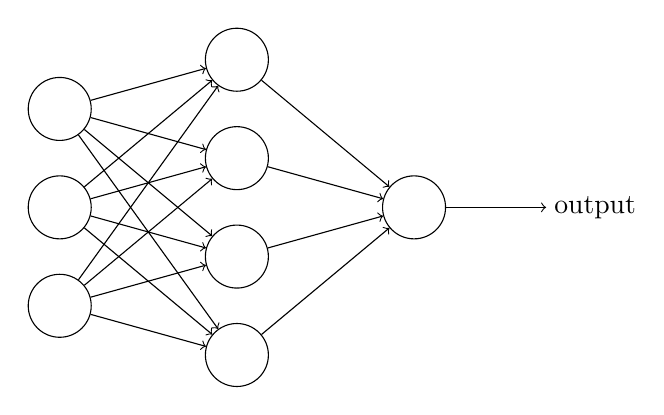
\begin{tikzpicture}
    [inner sep=0pt,minimum size=8mm]

    % leftmost neutrons:
    \node (pl1) at (-2.25, 1.25) [circle,draw] {};
    \node (pl2) at (-2.25, 0) [circle,draw] {};
    \node (pl3) at (-2.25, -1.25) [circle,draw] {};

    % middle neutrons:
    \node (pm1) at (0, 1.875) [circle,draw] {};
    \node (pm2) at (0, 0.625) [circle,draw] {};
    \node (pm3) at (0, -0.625) [circle,draw] {};
    \node (pm4) at (0, -1.875) [circle,draw] {};

    % rightmost neutron:
    \node (pr) at (2.25, 0) [circle,draw] {};

    % output:
    \node (output) at (4.5, 0) {\;output};

    % connect nodes:

    \draw [->] (pl1) to (pm1);
    \draw [->] (pl1) to (pm2);
    \draw [->] (pl1) to (pm3);
    \draw [->] (pl1) to (pm4);
    \draw [->] (pl2) to (pm1);
    \draw [->] (pl2) to (pm2);
    \draw [->] (pl2) to (pm3);
    \draw [->] (pl2) to (pm4);
    \draw [->] (pl3) to (pm1);
    \draw [->] (pl3) to (pm2);
    \draw [->] (pl3) to (pm3);
    \draw [->] (pl3) to (pm4);
    \draw [->] (pm1) to (pr);
    \draw [->] (pm2) to (pr);
    \draw [->] (pm3) to (pr);
    \draw [->] (pm4) to (pr);
    \draw [->] (pr) to (output);

  \end{tikzpicture}
\end{center}

之前提过,这个网络中最左边的称为输入层,其中的神经元称为输入神经元。最右边的,即
输出层包含有输出神经元,在本例中,输出层只有一个神经元。中间层,既然这层中的神经
元既不是输入也不是输出,则被称为隐藏层。``隐藏''这一术语也许听上去有些神秘 —— 我
第一次听到这个词,以为它必然有一些深层的哲学或数学涵意 —— 但它实际上仅仅意味着
``既非输入也非输出''。上面的网络仅有一个隐藏层,但有些网络有多个隐藏层。例如,下
面的四层网络有两个隐藏层:
% tikz11
\begin{center}
  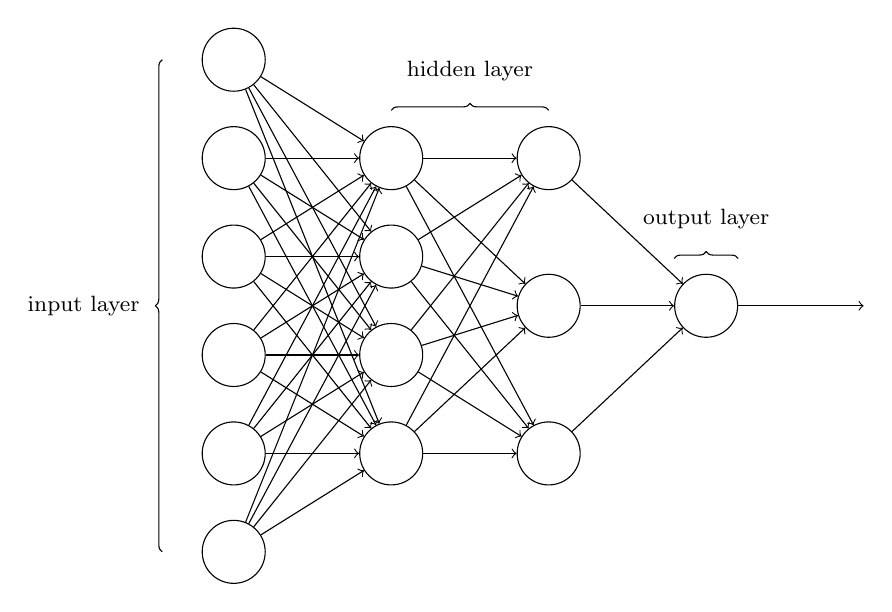
\begin{tikzpicture}
    [inner sep=0pt,minimum size=8mm]

    % leftmost neurons:
    \foreach \y in {0,...,5}
    \node (l\y) at (0, \y * 1.25) [circle,draw] {};

    % left hidden layers:
    \foreach \y in {0,...,3}
    \node (hl\y) at (2, \y * 1.25 + 1 * 1.25) [circle,draw] {};

    % right hidden layers:
    \foreach \y in {0,...,2}
    \node (hr\y) at (4, \y * 1.875 + 1 * 1.25) [circle,draw] {};

    % output:
    \node (output) at (6, 3.125) [circle,draw] {};

    % draw brace:
    \draw[decorate,decoration={brace,mirror}] ([xshift=-5mm]l5.west) -- ([xshift=-5mm]l0.west) node [midway,xshift=-10mm] {
      \footnotesize input layer
    };

    \draw[decorate,decoration={brace}] ([yshift=2mm]hl3.north) -- ([yshift=2mm]hr2.north) node [midway,yshift=5mm] {
      \footnotesize hidden layer
    };

    \draw[decorate,decoration={brace}] ([yshift=6mm]output.west) -- ([yshift=6mm]output.east) node [midway,yshift=5mm] {
      \footnotesize output layer
    };

    % connections:
    \foreach \x in {0,...,5}
    \foreach \y in {0,...,3}
    \draw [->] (l\x) to (hl\y);

    \foreach \x in {0,...,3}
    \foreach \y in {0,...,2}
    \draw [->] (hl\x) to (hr\y);

    \foreach \y in {0,...,2}
    \draw [->] (hr\y) to (output);

    \draw [->] (output) to (8, 3.125);

  \end{tikzpicture}
\end{center}

有些令人困惑的是,由于历史的原因,尽管是由S型神经元而不是感知器构成,这种多层网
络有时被称为多层感知器或者\emph{MLP}。在这本书中我不会使用 MLP 这个术语,因为我
认为这会引起混淆,但这里想提醒你它的存在。

设计网络的输入输出层通常是比较直接的。例如,假设我们尝试确定一张手写数字的图像上
是否写的是``9''。很自然地,我们可以将图片像素的强度进行编码作为输入神经元来设计
网络。如果图像是一个 $64 \times 64$ 的灰度图像,那么我们会需要 $4096 = 64 \times
64$ 个输入神经元,每个强度取 $0$ 和 $1$ 之间合适的值。输出层只需要包含一个神经元,
当输出值小于 $0.5$ 时表示 ``输入图像不是一个 $9$'',大于 $0.5$ 的值表示 ``输入图
像是一个 $9$''。

相比于神经网络中输入输出层的直观设计,隐藏层的设计则堪称一门艺术。特别是,通过一
些简单的经验法则来总结隐藏层的设计流程是不可行的。相反,神经网络的研究人员已经为
隐藏层开发了许多设计最优法则,这有助于网络的行为能符合人们期望的那样。例如,这些
法则可以用于帮助权衡隐藏层数量和训练网络所需的时间开销。在本书后面我们会碰到几个
这样的设计最优法则。

目前为止,我们讨论的神经网络,都是以上一层的输出作为下一层的输入。这种网络被称为
\emph{前馈}神经网络。这意味着网络中是没有回路的 —— 信息总是向前传播,从不反向回
馈。如果确实有回路,我们最终会有这样的情况:$\sigma$ 函数的输入依赖于输出。这将
难于理解,所以我们不允许这样的环路。

然而,也有一些人工神经网络的模型,其中反馈环路是可行的。这些模型被称为%
\href{http://en.wikipedia.org/wiki/Recurrent_neural_network}{递归神经网络}。这种
模型的设计思想,是具有休眠前会在一段有限的时间内保持激活状态的神经元。这种激活状
态可以刺激其它神经元,使其随后被激活并同样保持一段有限的时间。这样会导致更多的神
经元被激活,随着时间的推移,我们得到一个级联的神经元激活系统。因为一个神经元的输
出只在一段时间后而不是即刻影响它的输入,在这个模型中回路并不会引起问题。

递归神经网络比前馈网络影响力小得多,部分原因是递归网络的学习算法(至少目前为止)
不够强大。但是递归网络仍然很有吸引力。它们原理上比前馈网络更接近我们大脑的实际工
作。并且递归网络能解决一些重要的问题,这些问题如果仅仅用前馈网络来解决,则更加困
难。然而为了篇幅,本书将专注于使用更广泛的前馈网络。

\section{一个简单的分类手写数字的网络}

定义神经网络后,让我们回到手写识别上来。我们可以把识别手写数字的问题分成两个子问
题。首先,我们希望有个方式把包含许多数字的图像分成一系列单独的图像,每个包含单个
数字。例如,我们想要把图像
\begin{center}
  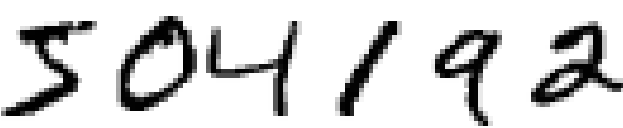
\includegraphics[width=64pt]{digits}
\end{center}
分成六个单独的图像,
\begin{center}
  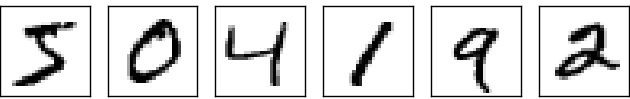
\includegraphics[height=32pt]{digits_separate}
\end{center}

我们人类可以很容易解决这个分割的问题,但是对于计算机程序来说却是个挑战。一旦图像
被分割,那么程序需要把每个单独的数字分类。例如,我们想要我们的程序能识别上面的第
一个数字
\begin{center}
  
\includegraphics[height=24pt]{mnist_first_digit}
\end{center}
是 $5$。

我们将专注于编程解决第二个问题,分类单独的数字。这样是因为,一旦你有分类单独数字
的有效方法,分割问题是不难解决的。有很多途径可以解决分割的问题。一种方法是尝试不
同的分割方式,用数字分类器对每一个切分片段打分。如果数字分类器对每一个片段的置信
度都比较高,那么这个分割方式就能得到较高的分数;如果数字分类器在一或多个片段中出
现问题,那么这种分割方式就会得到较低的分数。这种方法的思想是,如果分类器有问题,
那么很可能是由于图像分割出错导致的。这种思想以及它的变化形式能够比较好地解决分割
问题。因此,与其关心分割问题,我们不如把精力集中在设计一个神经网络来解决更有趣、
更困难的问题,即手写数字的识别。

我们将使用一个三层神经网络来识别单个数字:
% tikz12
\begin{center}
  \begin{tikzpicture}
    [inner sep=0pt,minimum size=5mm]

    % leftmost layer:
    \foreach \y in {1,...,8}
    \node (l\y) at (-4, 7.5 / 1.25 - 4 / 1.25 + \y / 1.25) [circle,draw] {};

    % hidden layer:
    \foreach \y in {1,...,15}
    \node (m\y) at (0, \y / 1.25) [circle,draw] {};

    % output layer:
    \foreach \y in {1,...,10}
    \node (r\y) at (4, 7.5 / 1.25 - 5 / 1.25 + \y / 1.25) [circle,draw] {};

    \foreach \y in {1,...,10}
    \node (o\y) [right=of r\y] {\footnotesize $\number \numexpr 10 -\y \relax$};

    \begin{scope}[node distance=2mm]
      \node (text1) [above=of m15] {
        \begin{tabular}{c}
          \footnotesize hidden layer \\
          \footnotesize ($n = 15$ neurons)
    	\end{tabular}
      };
      \node (text2) [above=of r10] {
        \footnotesize output layer
      };
    \end{scope}

    % draw brace:
    \draw[decorate,decoration={brace,mirror}] ([xshift=-5mm]l8.west) -- ([xshift=-5mm]l1.west) node [midway,xshift=-12.5mm] {
      \begin{tabular}{c}
        \footnotesize input layer \\
        \footnotesize ($784$ neurons)
      \end{tabular}
    };

    % connections:
    \foreach \x in {1,...,8}
    \foreach \y in {1,...,15}
    \draw [->] (l\x) to (m\y);

    \foreach \x in {1,...,15}
    \foreach \y in {1,...,10}
    \draw [->] (m\x) to (r\y);

    \foreach \x in {1,...,10}
    \draw [->] (r\x) to (o\x);

  \end{tikzpicture}
\end{center}

网络的输入层包含给输入像素的值进行编码的神经元。就像下一节会讨论的,我们给网络的
训练数据会有很多扫描得到的 $28 \times 28$ 的手写数字的图像组成,所有输入层包含有
$784 = 28 \times 28$ 个神经元。为了简化,上图中我已经忽略了 $784$ 中大部分的输入
神经元。输入像素是灰度级的,值为 $0.0$ 表示白色,值为 $1.0$ 表示黑色,中间数值表
示逐渐暗淡的灰色。

网络的第二层是一个隐藏层。我们用 $n$ 来表示神经元的数量,我们将给 $n$ 实验不同的
数值。示例中用一个小的隐藏层来说明,仅仅包含 $n=15$ 个神经元。

网络的输出层包含有 $10$ 个神经元。如果第一个神经元激活,即输出 $\approx 1$,那么
表明网络认为数字是一个 $0$。如果第二个神经元激活,就表明网络认为数字是一个 $1$。
依此类推。更确切地说,我们把输出神经元的输出赋予编号 $0$ 到 $9$,并计算出那个神
经元有最高的激活值。比如,如果编号为 $6$ 的神经元激活,那么我们的网络会猜到输入
的数字是 $6$。其它神经元相同。

你可能会好奇为什么我们用 $10$ 个输出神经元。毕竟我们的任务是能让神经网络告诉我们
哪个数字( $0, 1, 2, \ldots, 9$ )能和输入图片匹配。一个看起来更自然的方式就是使
用 $4$ 个输出神经元,把每一个当做一个二进制值,结果取决于它的输出更靠近 $0$ 还是
$1$~。四个神经元足够编码这个问题了,因为 $2^4 = 16$ 大于 $10$ 种可能的输入。为什
么我们反而要用 $10$ 个神经元呢?这样做难道效率不低吗?最终的判断是基于经验主义的:
我们可以实验两种不同的网络设计,结果证明对于这个特定的问题而言,$10$ 个输出神经
元的神经网络比4个的识别效果更好。但是令我们好奇的是为什么使用 $10$ 个输出神经元
的神经网络更有效呢。有没有什么启发性的方法能提前告诉我们用10个输出编码比使用 $4$
个输出编码更有好呢?

为了理解为什么我们这么做,我们需要从根本原理上理解神经网络究竟在做些什么。首先考
虑有 $10$ 个神经元的情况。我们首先考虑第一个输出神经元,它告诉我们一个数字是不是
0。它能那么做是因为可以权衡从隐藏层来的信息。隐藏层的神经元在做什么呢?假设隐藏
层的第一个神经元只是用于检测如下的图像是否存在:
\begin{center}
  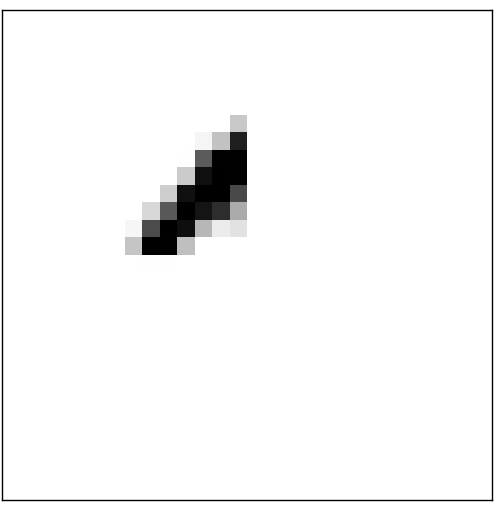
\includegraphics[height=32pt]{mnist_top_left_feature}
\end{center}

为了达到这个目的,它通过对此图像对应部分的像素赋予较大权重,对其它部分赋予较小的
权重。同理,我们可以假设第二,第三,第四个隐藏层的神经元是为检测下列图片是否存在:
\begin{center}
  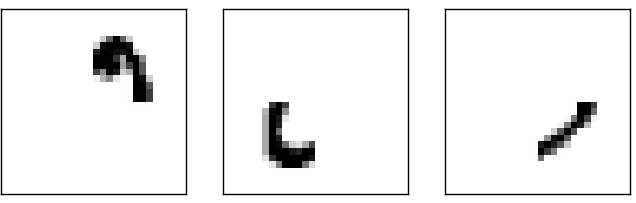
\includegraphics[height=32pt]{mnist_other_features}
\end{center}

就像你能猜到的,这四幅图像组合在一起构成了\hyperref[fig:digits]{之前}显示的一行
数字图像中的 $0$:
\begin{center}
  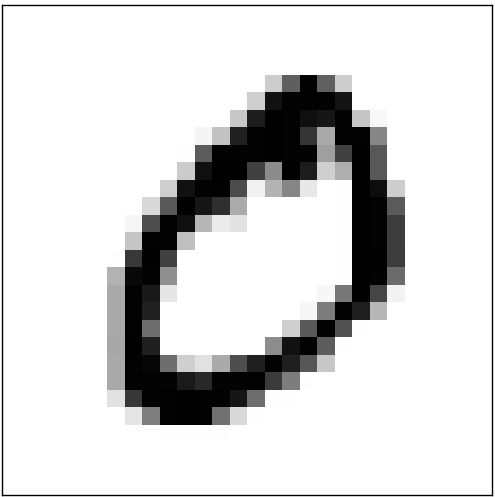
\includegraphics[height=32pt]{mnist_complete_zero}
\end{center}

如果所有这四个隐藏层的神经元被激活那么我们就可以推断出这个数字是 $0$。当然,这不
是我们推断出 $0$ 的唯一方式——我们能通过很多其他合理的方式得到 $0$ (举个例子来说,
  通过上述图像的转换,或者稍微变形)。但至少在这个例子中我们可以推断出输入的数字
是 $0$。

假设神经网络以上述方式运行,我们可以给出一个貌似合理的理由去解释为什么用 $10$ 个
输出而不是 $4$ 个。如果我们有 $4$ 个输出,那么第一个输出神经元将会尽力去判断数字
的最高有效位是什么。把数字的最高有效位和数字的形状联系起来并不是一个简单的问题。
很难想象出有什么恰当的历史原因,一个数字的形状要素会和一个数字的最高有效位有什么
紧密联系。

上面我们说的只是一个启发性的方法。没有什么理由表明这个三层的神经网络必须按照我所
描述的方式运行,即隐藏层是用来探测数字的组成形状。可能一个聪明的学习算法将会找到
一些合适的权重能让我们仅仅用4个输出神经元就行。但是这个启发性的方法通常很有效,
它会节省你大量时间去设计一个好的神经网络结构。

\subsection*{练习}

\begin{itemize}
\item 通过在上述的三层神经网络加一个额外的一层就可以实现按位表示数字。额外的一层
  把原来的输出层转化为一个二进制表示,如下图所示。为新的输出层寻找一些合适的权重
  和偏差。假定原先的3层神经网络在第三层得到正确输出(即原来的输出层)的激活值至
  少是 $0.99$,得到错误的输出的激活值至多是 $0.01$。
  \begin{center}
    \begin{tikzpicture}  %tikz13
      [inner sep=0pt,minimum size=5mm]

      % leftmost layer, 10 nodes:
      \foreach \y in {0,...,9}
      \node (l\y) at (-3, \y / 1.25) [circle,draw] {};

      % hidden layer, 5 nodes:
      \foreach \y in {0,...,4}
      \node (m\y) at (0, 2 + \y / 1.25) [circle,draw] {};

      % old output layer, 10 nodes:
      \foreach \y in {0,...,9}
      \node (r\y) at (3, \y / 1.25) [circle,draw] {};

      % new output layer, 4 nodes:
      \foreach \y in {0,...,3}
      \node (o\y) at (6, 2.4 + \y / 1.25) [circle,draw] {};

      % new output layer, 4 nodes:

      \foreach \y in {0,...,3}
      \node (a\y) [right=of o\y] {};

      \begin{scope}[node distance=3mm]
	\node (text2) [above=of r9] {
          \footnotesize old output layer
	};
      \end{scope}

      \begin{scope}[node distance=6mm]
	\node (text1) [above=of m4] {
          \footnotesize hidden layer
	};
	\node (text3) [above=of o3] {
          \footnotesize new output layer
	};
      \end{scope}

      % draw brace:
      \draw[decorate,decoration={brace,mirror}] ([xshift=-5mm]l9.west) -- ([xshift=-5mm]l0.west) node [midway,xshift=-12.5mm] {
        \begin{tabular}{c}
          \footnotesize input layer \\
          \footnotesize ($784$ neurons)
    	\end{tabular}
      };

      % connections:
      \foreach \x in {0,...,9}
      \foreach \y in {0,...,4}
      \draw [->] (l\x) to (m\y);

      \foreach \x in {0,...,4}
      \foreach \y in {0,...,9}
      \draw [->] (m\x) to (r\y);

      \foreach \x in {0,...,9}
      \foreach \y in {0,...,3}
      \draw [->] (r\x) to (o\y);

      \foreach \x in {0,...,3}
      \draw [->] (o\x) to (a\x);

    \end{tikzpicture}
  \end{center}
\end{itemize}

\section{使用梯度下降算法进行学习}

现在我们有了神经网络的设计,它怎样可以学习识别数字呢?我们需要的第一样东西是一个
用来学习的数据集 —— 称为训练数据集。我们将使用
\href{http://yann.lecun.com/exdb/mnist/}{MNIST 数据集},其包含有数以万计的连带着
正确分类器的手写数字的扫描图像。MNIST的名字来源于
\href{http://en.wikipedia.org/wiki/National_Institute_of_Standards_and_Technology}{NIST}
—— 美国国家标准与技术研究所 —— 收集的两个数据集改进后的子集。这是取自 MNIST 的一
些图像:
\begin{center}
  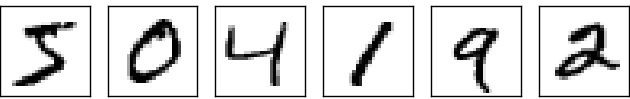
\includegraphics[height=32pt]{digits_separate}
\end{center}

正如你看到的,这些数字其实是和本章\hyperref[fig:digits]{开头}提到的一样。当然,
当测试我们的网络时我们将要求它识别不在训练集中的图像。

MNIST 数据分为两个部分。第一部分包含 60,000 幅用于训练数据的图像。这些图像扫描自
250 人的手写样本,他们中一半人是美国人口普查局的员工,一半人是高校学生。这些图像
是 $28 \times 28$ 大小的灰度图像。第二部分是 10,000 幅用于测试数据的图像,同样是
$28 \times 28$ 的灰度图像。我们将用这些测试数据来评估我们的神经网络学会识别数字
有多好。为了让其有好的的测试表现,测试数据取自和原始训练数据不同的\emph{另外}一
组 250 人(尽管仍然分别是美国人口普查局和高校学生)。这有助于确保我们的系统能识
别那些没有看到训练数据的人写的数字。

我们将用符号 $x$ 来表示一个训练输入。为了方便,把每个训练输入 $x$ 看作一个 $28
\times 28 = 784$ 维的向量。每个向量中的项目代表图像中单个像素的灰度值。我们用 $y
= y(x)$ 表示对应的期望输出,这里 $y$ 是一个 $10$ 维的向量。例如,如果有一个特定
的画成 $6$ 的训练图像,$x$,那么 $y(x) = (0, 0, 0, 0, 0, 0, 1, 0, 0, 0)^T$ %则是
网络的期望输出。注意这里 $T$ 是转置操作,把一个行向量转换成一个列向量。

我们希望有一个算法,能让我们找到权重和偏差,以至于网络的输出 $y(x)$ 能够拟合所有
的训练输入$x$。为了量化我们如何实现这个目标,我们定义一个\emph{代价函
  数}\footnote{有时被称为\emph{损失}或\emph{目标}函数。我们在这本书中使用了代价
  函数这个术语,但是你应该注意其他的术语,因为它经常被用于研究论文和其他神经网络
  的讨论中。}:
\begin{equation}
  C(w,b) \equiv \frac{1}{2n} \sum_x \| y(x) - a\|^2
  \label{eq:6}\tag{6}
\end{equation}

这里 $w$ 表示所有的网络中权重的集合,$b$ 是所有的偏差,$n$ 是训练输入数据的个数,
$a$ 是表示当输入为 $x$ 时输出的向量,求和则是在总的训练输入 $x$ 上进行的。当然,
输出 $a$ 取决于 $x$, $w$ 和 $b$,但是为了保持符号的简洁性,我没有明确地指出这种
依赖关系。符号 $\|v\|$ 是指向量 $v$ 的模。我们把 $C$ 称为\emph{二次代价函数};有
时也称被称为\emph{均方误差}或者\emph{MSE}。观察二次代价函数的形式我们可以看到
$C(w,b)$ 是非负的,因为求和公式中的每一项都是非负的。此外,代价函数 $C(w,b)$的值
相当小,即 $C(w,b) \approx 0$,精确地说,是当对于所有的训练输入 $x$,$y(x)$接近
于输出 $a$ 时。因此如果我们的学习算法能找到合适的权重和偏差,使得 $C(w,b)
\approx 0$,它就能很好地工作。相反,当 $C(w,b)$ 很大时就不怎么好了,那意味着对于
大量地输入, $y(x)$ 与输出 $a$ 相差很大。因此我们的训练算法的目的,是最小化权重
和偏差的代价函数 $C(w,b)$。换句话说,我们想要找到一系列能让代价尽可能小的权重和
偏差。我们将采用称为\emph{梯度下降}的算法法来达到这个目的。

为什么要介绍二次代价呢?毕竟我们最初感兴趣的内容不是能正确分类的图像数量吗?为什
么不试着直接最大化这个数量,而是去最小化一个类似二次代价的间接评量呢?这么做是因
为在神经网络中,被正确分类的图像数量所关于权重和偏差的函数并不是一个平滑的函数。
大多数情况下,对权重和偏差做出的微小变动完全不会影响被正确分类的图像的数量。这会
导致我们很难去解决如何改变权重和偏差来取得改进的性能。而用一个类似二次代价的平滑
代价函数则能更好地去解决如何用权重和偏差中的微小的改变来取得更好的效果。这就是为
什么我们首先专注于最小化二次代价,只有这样,我们之后才能测试分类精度。

即使已经知道我们需要使用一个平滑的代价函数,你可能仍然想知道为什么我们在方
程~\eqref{eq:6} 中选择二次函数。这是临时想出来的吗?是不是我们选择另一个不同的代
价函数将会得到完全不同的最小化的权重和偏差呢?这种顾虑是合理的,我们后面会再次回
到这个代价函数,并做一些修改。尽管如此,方程~\eqref{eq:6} 中的二次代价函数让我们
更好地理解神经网络中学习算法的基础,所以目前我们会一直使用它。

重复一下,我们训练神经网络的目的是找到能最小化二次代价函数 $C(w,b)$ 的权重和偏差。
这是一个适定问题,但是现在它有很多让我们分散精力的结构 —— 对权重 $w$ 和偏差 $b$
的解释,晦涩不清的 $\sigma$ 函数,神经网络结构的选择,MNIST 等等。事实证明我们可
以忽略结构中大部分,把精力集中在最小化方面来理解它。现在我们打算忘掉所有关于代价
函数的具体形式、神经网络的连接等等。现在让我们想象只要最小化一个给定的多元函数。
我们打算使用一种被称为\emph{梯度下降}的技术来解决这样的最小化问题。然后我们回到
在神经网络中要最小化的特定函数上来。

好了,假设我们要最小化某些函数,$C(v)$。它可以是任意的多元实值函数,$v = v_1,
v_2, \ldots$。注意我们用 $v$ 代替了 $w$ 和 $b$ 以强调它可能是任意的函数 —— 我们
现在先不局限于神经网络的环境。为了最小化 $C(v)$,想象 $C$ 是一个只有两个变量
$v1$和 $v2$ 的函数:
\begin{center}
  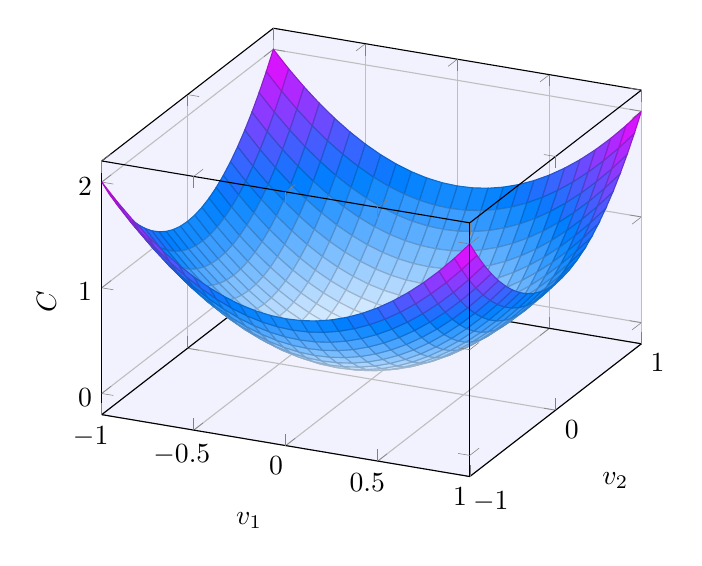
\begin{tikzpicture}
    % FIXME: rotate the zlabel, change plot color, and move z axis to right
    \begin{axis}[
      %title={$x^2 + y^2$},
      3d box=complete,
      grid=major,
      axis background/.style={fill=blue!5},
      xlabel=$v_1$,
      ylabel=$v_2$,
      zlabel=$C$,
      colormap/cool]
      \addplot3[surf,domain=-1:1] {
        x*x + y*y
      };
    \end{axis}
  \end{tikzpicture}
\end{center}

我们想要的是找到 $C$ 的全局最小值。当然,对于上图的函数,我们一眼就能找到最小值。
那只意味着,也许我展示的函数\emph{过于}简单了!通常函数 $C$ 可能是一个复杂的多元
函数,看一下就能找到最小值可是不可能的。

一种解决这个问题的方式是用微积分来解析最小值。我们可以计算导数去寻找 $C$ 的极值
点。运气好的话,$C$ 是一个只有一个或少数几个变量的函数。但是变量过多的话那就是噩
梦。而且神经网络中我们经常需要\emph{大量}的变量——最大的神经网络有依赖数亿权重和
偏差的代价函数,极其复杂。用微积分来计算最小值已经不可行了。

(确定我们将可以通过有两个变量的函数 $C$ 来理解神经网络后,我已经两次提到:``嘿,
  如果函数有远多于两个变量怎么办?''。对此我只能说很抱歉。请相信我把 $C$ 想象成
  一个二元函数是有助于我们的理解的。有时候这种想象的画面会遇到障碍,这正是上面两
  个段落在帮助你克服的。善于思考数学通常也涉及到有效地利用多种直觉上的想象画面,
  学会什么时候用什么画面合适。)

好吧,微积分是不能用了。幸运的是,有一个漂亮的推导法暗示有一种算法能得到很好的效
果。首先把我们的函数想象成一个山谷。只要瞄一眼上面的绘图就不难理解。我们想象有一
个小球从山谷的斜坡滚落下来。我们的日常经验告诉我们这个球最终会滚到谷底。也许我们
可以用这一想法来找到函数的最小值?我们会为一个(假想的)球体随机选择一个起始位置,
然后模拟球体滚落到谷底的运动。我们可以通过计算 $C$ 的导数(或者二阶导数)来简单
模拟——这些导数会告诉我们山谷中局部``形状''的一切,由此知道我们的球将怎样滚动。

看到这里你可能会以为我们会写下球体的牛顿运动定理,考虑摩擦力、重力等影响。实际上,
我们不打算真的去实现这个球体滚落的推导 —— 我们是在设计一个最小化 $C$ 的算法,而
不是在用物理定律做精确的仿真。对球体的肉眼观察是为了激发我们的想象而不是束缚我们
的思维。因此与其陷进物理学里凌乱的细节,不如我们就这样问自己:如果我们扮演一天的
上帝,能够构造自己的物理定律,能够支配球体可以如何滚动,那么我们将会采取什么样的
运动学定律来让球体能够总是滚落到谷底呢?

为了更精确地描述这个问题,让我们思考一下,当我们在 $v1$ 和 $v2$ 方向分别将球体移
动一个很小的量,即 $\Delta v1$ 和 $\Delta v2$ 时,球体将会发生什么情况。微积分告
诉我们 $C$ 将会有如下变化:
\begin{equation}
  \Delta C \approx \frac{\partial C}{\partial v_1} \Delta v_1 +
  \frac{\partial C}{\partial v_2} \Delta v_2
  \label{eq:7}\tag{7}
\end{equation}

我们要寻找一种选择 $\Delta v_1$ 和 $\Delta v_2$ 的方法使得 $\Delta C$ 为负;即,
我们选择它们是为了让球体滚落。为了弄明白如何选择,需要定义 $\Delta v$ 为 $v$ 变
化的向量,$\Delta v \equiv (\Delta v_1, \Delta v_2)^T$,$T$ 是转置符号。我们也定
义 $C$ 的梯度为偏导数的向量,$\left(\frac{\partial C}{\partial v_1},
\frac{\partial C}{\partial v_2}\right)^T$。我们用 $\nabla C$ 来表示梯度向量,即:
\begin{equation}
  \nabla C \equiv \left( \frac{\partial C}{\partial v_1}, \frac{\partial
      C}{\partial v_2} \right)^T
  \label{eq:8}\tag{8}
\end{equation}

我们马上会用 $\Delta v$ 和梯度 $\nabla C$ 来重写 $\Delta C$ 的变化。在这之前我想
先澄清一些令人困惑的关于梯度的事情。当第一次碰到 $\nabla C$ 这个符号,人们有时会
想知道怎么去理解 $\nabla$ 符号。$\nabla$ 究竟是什么意思?事实上你可以把 $\nabla
C$ 仅仅看做一个简单的数学记号 —— 上面定义的向量 —— 这样就不必写两个符号了。这样
来看,$\nabla$ 仅仅是一个符号,犹如风中摆动的旗帜,告诉你:``嘿,$\nabla C$ 是一
个梯度向量''。也有很多其它的数学上不同视角对于 $\nabla$ 的专业解释(比如,作为一
  个微分操作),但我们不需要这些观点。

有了这些定义,$\Delta C$ 的表达式~\eqref{eq:7} 可以被重写为:
\begin{equation}
  \Delta C \approx \nabla C \cdot \Delta v
  \label{eq:9}\tag{9}
\end{equation}

这个表达式解释了为什么 $\nabla C$ 被称为梯度向量:$\nabla C$ 把 $v$ 的变化关联为
$C$ 的变化,正如我们期望的用梯度来表示。但是这个方程真正让我们兴奋的是它让我们看
到了如何选取 $\Delta v$ 才能让 $\Delta C$ 为负数。假设我们选取:
\begin{equation}
  \Delta v = -\eta \nabla C
  \label{eq:10}\tag{10}
\end{equation}

这里的 $\eta$ 是个很小的正数(称为\emph{学习速率})。方程~\eqref{eq:9} 告诉我们
$\Delta C \approx -\eta \nabla C \cdot \nabla C = -\eta \|\nabla C\|^2$。由于
$\| \nabla C \|^2 \geq 0$,这保证了$\Delta C \leq 0$,即,如果我们按照方
程~\eqref{eq:10} 的规则去改变 $v$,那么 $C$ 会一直减小,不会增加。(当然,要在方
  程~\eqref{eq:9}的近似约束下)。这正是我们想要的特性!因此我们把方
程~\eqref{eq:10} 用于定义球体在梯度下降算法下的“运动定律”。也就是说,我们用方
程~\eqref{eq:10} 计算 $\Delta v$,来移动球体的位置 $v$:
\begin{equation}
  v \rightarrow v' = v -\eta \nabla C
  \label{eq:11}\tag{11}
\end{equation}

然后我们用它再次更新规则来计算下一次移动。如果我们反复持续这样做,我们将持续减小
$C$ 直到 —— 正如我们希望的 —— 获得一个全局的最小值。

总结一下,梯度下降算法工作的方式就是重复计算梯度 $\nabla C$,然后沿着\emph{相反}
的方向移动,沿着山谷``滚落''。我们可以想象它像这样:
\begin{center}
  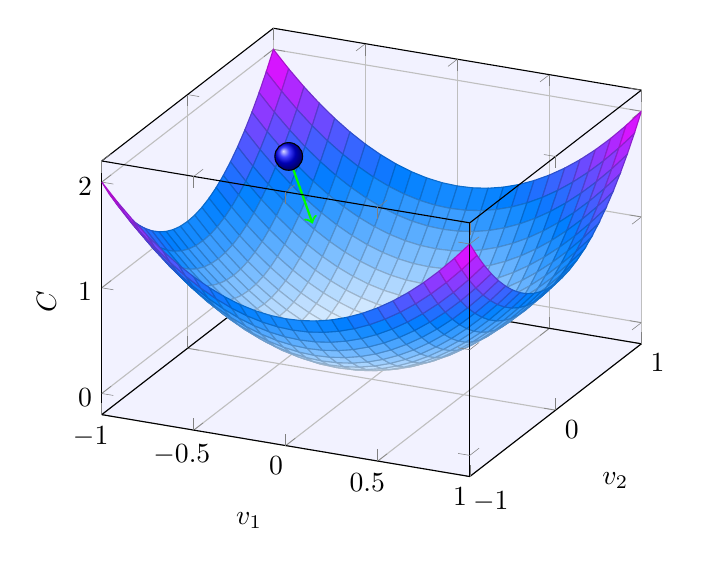
\begin{tikzpicture}
    % FIXME: rotate the zlabel, change plot color, and move z axis to right
    \begin{axis}[
      %title={$x^2 + y^2$},
      3d box=complete,
      grid=major,
      axis background/.style={fill=blue!5},
      xlabel=$v_1$,
      ylabel=$v_2$,
      zlabel=$C$,
      colormap/cool]

      \addplot3[surf,domain=-1:1] {
        x*x + y*y
      };

      \addplot3[mark=ball,mark size=5pt] coordinates {
        (-0.8, 0.75, 1.2025)
      };

      \draw[->,thick,green] (axis cs:-0.8,0.75,1.2025) -- (axis cs:-0.6, 0.6, 0.72);

    \end{axis}
  \end{tikzpicture}
\end{center}

注意具有这一规则的梯度下降并不是模仿实际的物理运动。在现实中一个球体有动量,使得
它岔开斜坡滚动,甚至(短暂地)往山上滚。只有在克服摩擦力的影响,球体才能保证滚到
山谷。相比之下,我们选择 $\Delta v$ 规则只是说:``往下,现在''。这仍然是一个寻找
最小值的非常好的规则!

为了使梯度下降能够正确地运行,我们需要选择足够小的学习速率 $\eta$ 使得方
程~\eqref{eq:9} 能得到很好的近似。如果不这样,我们会以 $\Delta C > 0$ 结束,这显
然不好。同时,我们也不想 $\eta$ 太小,因为这会使 $\Delta v$ 的变化极小,梯度下降
算法就会运行得非常缓慢。在真正的实现中,$\eta$ 通常是变化的,以至方
程~\eqref{eq:9}能保持很好的近似度,但算法又不会太慢。我们后面会看这是如何工作的。

我已经解释了具有两个变量的函数 $C$ 的梯度下降。但事实上,即使 $C$ 是一个具有更多
变量的函数也能很好地工作。我们假设 $C$ 是一个有 $m$ 个变量 $v_1,\ldots,v_m$ 的多
元函数。那么对 $C$ 中自变量的变化 $\Delta v = (\Delta v_1, \ldots, \Delta
v_m)^T$,$\Delta C$ 将会变为:
\begin{equation}
  \Delta C \approx \nabla C \cdot \Delta v
  \label{eq:12}\tag{12}
\end{equation}

这里的梯度 $\nabla C$ 是向量
\begin{equation}
  \nabla C \equiv \left(\frac{\partial C}{\partial v_1}, \ldots,
    \frac{\partial C}{\partial v_m}\right)^T
  \label{eq:13}\tag{13}
\end{equation}

正如两个变量的情况,我们可以选取
\begin{equation}
  \Delta v = -\eta \nabla C
  \label{eq:14}\tag{14}
\end{equation}

而且 $\Delta C$ 的(近似)表达式~\eqref{eq:12} 保证是负数。这给了我们一种方式从
梯度中去取得最小值,即使 $C$ 是任意的多元函数,我们也能重复运用更新规则
\begin{equation}
  v \rightarrow v' = v-\eta \nabla C
  \label{eq:15}\tag{15}
\end{equation}

你可以把这个更新规则看做\emph{定义}梯度下降算法。这给我们提供了一种方式去通过重
复改变 $v$ 来找到函数 $C$ 的最小值。这个规则并不总是有效的 —— 有几件事能导致错误,
让我们无法从梯度下降来求得函数 $C$ 的全局最小值,这个观点我们会在后面的章节中去
探讨。但在实践中,梯度下降算法通常工作地非常好,在神经网络中这是一种非常有效的方式
去求代价函数的最小值,进而促进网络自身的学习。

事实上,甚至有一种观点认为梯度下降法是求最小值的最优策略。假设我们正在努力去改变
$\Delta v$ 来让 $C$ 尽可能地减小。这相当于最小化$\Delta C \approx \nabla C \cdot
\Delta v$。我们首先限制步长为小的固定值,即$\| \Delta v \| = \epsilon$,
$\epsilon > 0$。当步长固定时,我们要找到使得 $C$ 减小最大的下降方向。可以证明,
使得 $\nabla C \cdot \Delta v$ 取得最小值的 $\Delta v$ 为 $\Delta v = - \eta
\nabla C$,这里 $\eta = \epsilon / \|\nabla C\|$ 是由步长限制 $\|\Delta v\| =
\epsilon$ 所决定的。因此,梯度下降法可以被视为一种在 $C$下降最快的方向上做微小变
化的方法。

\subsection*{练习}

\begin{itemize}
\item 证明上一段落的推断。提示:可以利用
  \href{http://en.wikipedia.org/wiki/Cauchy–Schwarz_inequality}{柯西-施瓦茨不等
    式}。
\item 我已经解释了当 $C$ 是二元及其多元函数的情况。那如果 $C$ 是一个一元函数呢?
  你能给出梯度下降法在一元函数的几何解释么?
\end{itemize}

人们已经研究出很多梯度下降的变化形式,包括一些更接近真实模拟球体物理运动的变化形
式。这些模拟球体的变化形式有很多优点,但是也有一个主要的缺点:它最终必需去计算
$C$ 的二阶偏导,这代价可是非常大的。为了理解为什么这种做法代价高,假设我们想求所
有的二阶偏导 $\partial^2 C/ \partial v_j \partial v_k$。如果我们有上百万的变量
$v_j$,那我们必须要计算数万亿(即百万次的平方)级别的二阶偏导\footnote{实际上,
  更接近万亿次的一半,因为$\partial^2 C/ \partial v_j \partial v_k = \partial^2
  C/ \partial v_k \partial v_j$。同样,你知道怎么做。}!这会造成很大的计算代价。
不过也有一些避免这类问题的技巧,寻找梯度下降算法的替代品也是个很活跃的研究领域。
但在这本书中我们将主要用梯度下降算法(包括变化形式)使神经网络学习。

我们怎么在神经网络中用梯度下降算法去学习呢?其思想就是利用梯度下降算法去寻找能使
得方程~\eqref{eq:6} 的代价取得最小值的权重 $w_k$ 和偏差 $b_l$。为了清楚这是如何工
作的,我们将用权重和偏差代替变量 $v_j$。也就是说,现在``位置''变量有两个分量组
成:$w_k$ 和 $b_l$,而梯度向量 $\nabla C$ 则有相应的分量 $\partial C / \partial
w_k$和$\partial C / \partial b_l$。用这些分量来写梯度下降的更新规则,我们得到:
\begin{align}
  \label{eq:16}w_k \rightarrow w_k' &= w_k-\eta \frac{\partial C}{\partial w_k}\tag{16}\\
  \label{eq:17}b_l \rightarrow b_l' &= b_l-\eta \frac{\partial C}{\partial b_l}\tag{17}
\end{align}

通过重复应用这一更新规则我们就能``让球体滚下山'',并且有望能找到代价函数的最小值。
换句话说,这是一个能让神经网络学习的规则。

应用梯度下降规则有很多挑战。我们将在下一章深入讨论。但是现在只提及一个问题。为了
理解问题是什么,我们先回顾\eqref{eq:6} 中的二次代价。注意这个代价函数有着这样的形
式 $C = \frac{1}{n} \sum_x C_x$,即,它是遍及每个训练样本代价 $C_x \equiv
\frac{\|y(x)-a\|^2}{2}$ 的平均值。在实践中,为了计算梯度 $\nabla C$,我们需要为每
个训练输入 $x$ 单独地计算梯度值 $\nabla
C_x$,然后求平均值,$\nabla C = \frac{1}{n} \sum_x \nabla C_x$。不幸的是,当训练
输入的数量过大时会花费很长时间,这样会使学习变得相当缓慢。

有种叫做\emph{随机梯度下降}的算法能够加速学习。其思想就是通过随机选取小量训练输
入样本来计算 $\nabla C_x$,进而估算梯度 $\nabla C$。通过计算少量样本的平均值我们
可以快速得到一个对于实际梯度 $\nabla C$ 的很好的估算,这有助于加速梯度下降,进而
加速学习过程。

更准确地说,随机梯度下降通过随机选取小量的 $m$ 个训练输入来工作。我们将这些随机
的训练输入标记为$X_1, X_2, \ldots, X_m$,并把它们称为一个\emph{小批量输入
  (mini-batch)}\footnote{译注:学习算法通常都是一批一批选取输入,可以是一个
  mini-batch, 也可以是一个 full-batch,重要的是权衡精度和时间选择合适的 batch
  size。因此本文将 mini-batch 按照上下文翻译为小批量输入、小批量数据等,在后面的
  代码中你也会看到 mini\_batch 变量,这些都是一个意思。}。假设样本数量 $m$ 足够
大,我们期望 $\nabla C_{X_j}$ 的平均值大致相等于整个 $\nabla C_x$ 的平均值,即,
\begin{equation}
  \frac{\sum_{j=1}^m \nabla C_{X_{j}}}{m} \approx \frac{\sum_x \nabla C_x}{n} = \nabla C
  \label{eq:18}\tag{18}
\end{equation}

这里的第二个求和符号是在整个训练数据上进行的。交换两边我们得到
\begin{equation}
  \nabla C \approx \frac{1}{m} \sum_{j=1}^m \nabla C_{X_{j}}
  \label{eq:19}\tag{19}
\end{equation}
证实了我们可以通过仅仅计算随机选取的小批量数据的梯度来估算整体的梯度。

为了将其明确地和神经网络的学习联系起来,假设 $w_k$ 和 $b_l$ 表示我们神经网络中权
重和偏差。随即梯度下降通过随机地选取并训练小批量的输入来工作,
\begin{align}
  \label{eq:20}w_k \rightarrow w_k' &= w_k-\frac{\eta}{m}
                                      \sum_j \frac{\partial C_{X_j}}{\partial w_k}
                                      \tag{20}\\
  \label{eq:21}b_l \rightarrow b_l' &= b_l-\frac{\eta}{m}
                                      \sum_j \frac{\partial C_{X_j}}{\partial b_l}
                                      \tag{21}
\end{align}
其中两个求和符号是在当前小批量输入中的所有训练样本 $X_j$ 上进行的。然后我们再挑选另一随机
选定的小批量输入去训练。直到我们用完了所有的训练输入,这被称为完成了一个训练%
\emph{周期(epoch)}\footnote{译注:英文为 epoch,本书中统一称之为``训练周期'',
  因为它就是指训练程序的一次完整的迭代,即当所有的输入变量都在训练算法中用到时,
  一个 epoch 就完成了。但请记住 epoch 这个单词,在一些神经网络分析软件(例如
    MATLAB)中,你会经常看到用户可输入的 epoch 参数。
% 参考 http://stackoverflow.com/questions/25887205/what-is-an-epoch-in-anns-and-how-does-it-translate-into-code-in-matlab
}。然后我们就会开始一个新训练周期。

% In the neural network terminology:
%
% one epoch = one forward pass and one backward pass of all the training
% examples
%
% batch size = the number of training examples in one forward/backward pass. The
% higher the batch size, the more memory space you'll need.
%
% number of iterations = number of passes, each pass using [batch size] number
% of examples. To be clear, one pass = one forward pass + one backward pass (we
% do not count the forward pass and backward pass as two different passes).
%
% Example: if you have 1000 training examples, and your batch size is 500, then
% it will take 2 iterations to complete 1 epoch.
%
% and: http://stackoverflow.com/questions/25887205/what-is-an-epoch-in-anns-and-how-does-it-translate-into-code-in-matlab

另外值得提一下,对于改变代价函数大小的参数,和用于计算权重和偏差的小批量输入的更
新规则,会有不同的约定。在方程~\eqref{eq:6} 中,我们通过因子$\frac{1}{n}$ 来改变
整个代价函数的大小。人们有时候忽略
$\frac{1}{n}$,直接取单个训练样本的代价总和,而不是取平均值。这对我们不能提前知道
训练数据数量的情况下特别有效。例如,这可能发生在有更多的训练数据是实时产生的情况
下。同样,小批量输入的更新规则~\eqref{eq:20} 和~\eqref{eq:21} 有时也会舍弃前面
的 $\frac{1}{m}$。从概念上这会有一点区别,因为它等价于改变了学习速率 $\eta$ 的大
小。但在对不同工作进行详细对比时,需要对它警惕。

我们可以把随机梯度下降想象成一次民意调查:在一个小批量上采样比对一个完整数据集进
行梯度下降分析要容易得多,正如进行一次民意调查比举行一次全民选举要更容易。例如,
如果我们有一个规模为 $n = 60,000$ 的训练集,就像 MNIST,并选取小批量数据大小
为 $m = 10$,这意味着在估算梯度过程中加速了 $6,000$ 倍!当然,这个估算并不是完美
的 —— 存在统计波动 —— 但是没必要完美:我们实际关心的是在某个方向上移动来减少
$C$,而这意味着我们不需要梯度的精确计算。在实践中,随机梯度下降是在神经网络的学习
中被广泛使用、十分有效的技术,它也是本书中展开的大多数学习技术的基础。

\subsection*{练习}

\begin{itemize}
\item 梯度下降算法一个极端的版本是把小批量输入的大小设为 $1$。即,假设一个训练输
  入 $x$,我们按照规则 $w_k \rightarrow w_k' = w_k - \eta \partial C_x /
  \partial w_k$和$b_l \rightarrow b_l' = b_l - \eta \partial C_x / \partial b_l$
  更新我们的权重和偏差。然后我们选取另一个训练输入,再一次更新权重和偏差。如此重
  复。这个过程被称为 \emph{online}、\emph{on-line}、或者\emph{递增}学习。在递增
  学习中,神经网络在一个时刻只学习一个训练输入(正如人类做的)。对比具有一个小批
  量输入大小为 $20$ 的随机梯度下降,说出递增学习的一个优点和一个缺点。
\end{itemize}

让我们讨论一个令刚接触梯度下降的人困惑的问题来总结这部分的内容。在神经网络中,代
价函数 $C$ 是一个关于所有权重和偏差的多元函数,因此在某种意义上来说,就是在一个
高维空间定义了一个平面。有些人可能会担心地想:``嘿,我必须要想象其它多出的维度''。
他们会开始发愁:``我不能想象出四维空间,更不用说五维(或者五百万维)''。是不是他
们缺少某种只有``超级''数学家才有的超能力?当然不是。即使大多数专业的数学家也不能
想象出四维空间的样子。他们用的技巧,是扩展出其它的方法来描绘发生了什么事。正如我
们上面所做的那样,我们用代数(而不是图像)描绘 $\Delta C$ 来计算如何变化才能让
$C$ 减少。那些善于思考高维的人内心有着包含有许多不同的技术的知识库;我们的代数技
巧也是一个例子。这些技术可能没有我们习惯于思考三维时的那么简单,但一旦你构建起这
样的知识库,你能够更从容应对更高的维度。我不想在这里详细展开,如果你感兴趣,你可
以阅读这个关于专业的数学家如何思考高维空间
的%
\href{http://mathoverflow.net/questions/25983/intuitive-crutches-for-higher-dimensional-thinking}{
  讨论}。我们讨论的一些技术可能会有点复杂,但很多最好的内容还是比较直观并容易理
解的,任何人都能熟练掌握。

\section{实现我们的网络来分类数字}
\label{sec:implementing_our_network_to_classify_digits}

好吧,现在让我们写一个学习如何识别手写数字的程序,使用随机梯度下降算法和 MNIST 训
练数据。我们需要做的第一件事情是获取 MNIST 数据。如果你是一个 \lstinline!git! 用
户,那么你能够通过克隆这本书的代码仓库获得数据,

\begin{lstlisting}[language=sh]
git clone https://github.com/mnielsen/neural-networks-and-deep-learning.git
\end{lstlisting}

如果你不使用 \lstinline!git!,也可以从%
\href{https://github.com/mnielsen/neural-networks-and-deep-learning/archive/master.zip}{
  这里}下载数据和代码。

顺便提一下,当我在之前描述 MNIST 数据时,我说它分成了 60,000 个训练图像
和 10,000个测试图像。这是官方的 MNIST 的描述。实际上,我们将用稍微不同的方法对数
据进行划分。我们将测试集保持原样,但是将 60,000 个图像的 MNIST 训练集分成两个部分:
一部分 50,000 个图像,我们将用来训练我们的神经网络,和一个单独的 10,000 个图像
的\emph{验证集}。在本章中我们不使用验证数据,但是在本书的后面我们将会发现它对于解
决如何去设置某些神经网络中的\emph{超参数}\index{超参数}是很有用的 —— 例如学习速率等,这些参数不
被我们的学习算法直接选择。尽管验证数据不是原始 MNIST 规范的一部分,然而许多人以这
种方式使用 MNIST,并且在神经网络中使用验证数据是很普遍的。从现在起当我提
到``MNIST 训练数据''时,我指的是我们的 50,000 个图像数据集,而不是原始的 60,000
图像数据集\footnote{如前所述,MNIST数据集是基于NIST(美国国家标准与技术研究院)收
  集的两个数据集合。为了构建MNIST,NIST数据集合被Yann LeCun,Corinna
  Cortes和Christopher J. C. Burges拆分放入一个更方便的格式。更多细节请看这个链接。
  我的仓库中的数据集是在一种更容易在Python中加载和操纵MNIST数据的形式。我从蒙特利
  尔大学的LISA机器学习实验室获得了这个特殊格式的数据
  (\href{http://www.deeplearning.net/tutorial/gettingstarted.html}{链接})}。

除了 MNIST 数据,我们还需要一个叫做 \href{http://numpy.org/}{Numpy} 的 Python 库,
用来做快速线性代数。如果你没有安装过 Numpy,你能够
从\href{http://www.scipy.org/install.html}{这里}下载。

在列出一个完整的代码清单之前,让我解释一下神经网络代码的核心特性。核心片段是一
个 \lstinline!Network! 类,我们用来表示一个神经网络。这是我们用来初始化一
个 \lstinline!Network! 对象的代码:
\begin{lstlisting}[language=Python]
class Network(object):

	def __init__(self, sizes):
		self.num_layers = len(sizes)
		self.sizes = sizes
		self.biases = [np.random.randn(y, 1) for y in sizes[1:]]
		self.weights = [np.random.randn(y, x)
						for x, y in zip(sizes[:-1], sizes[1:])]
\end{lstlisting}

在这段代码中,列表 \lstinline!sizes! 包含各层神经元的数量。例如,如果我们想创建
一个在第一层有 2 个神经元,第二层有 3 个神经元,最后层有 1 个神经元的
\lstinline!Network! 对象,我们应这样写代码:
\begin{lstlisting}[language=Python]
net = Network([2, 3, 1])
\end{lstlisting}

\lstinline!Network! 对象中的偏差和权重都是被随机初始化的,使用 Numpy 的
\lstinline!np.random.randn! 函数来生成均值为 0,标准差为 1 的高斯分布。这样的随
机初始化给了我们的随机梯度下降算法一个起点。在后面的章节中我们将会发现更好的初始
化权重和偏差的方法,但是目前随机地将其初始化。注意 \lstinline!Network! 初始化代
码假设第一层神经元是一个输入层,并对这些神经元不设置任何偏差,因为偏差仅在后面的
层中用于计算输出。

另外注意,偏差和权重以 Numpy 矩阵列表的形式存储。例如 \lstinline!net.weights[1]!
是一个存储着连接第二层和第三层神经元权重的 Numpy 矩阵。(不是第一层和第二层,因
  为 Python 列表的索引从 0 开始。)既然 \lstinline!net.weights[1]! 相当冗长,让
我们用 $w$ 表示矩阵。矩阵的 $w_{jk}$ 是连接第二层的 $k^{\rm th}$ 神经元和第三层
的 $j^{\rm th}$ 神经元的权重。这种 $j$ 和 $k$ 索引的顺序可能看着奇怪 —— 交换 $j$
和 $k$ 索引会更有意义,确定吗?使用这种顺序的很大的优势是它意味着第三层神经元的
激活向量是:
\begin{equation}
  a' = \sigma(w a + b)
  \label{eq:22}\tag{22}
\end{equation}

这个方程有点奇怪,所以让我们一块一块地理解它。$a$ 是第二层神经元的激活向量。为了
得到 $a'$,我们用权重矩阵 $w$ 乘以 $a$,加上偏差向量 $b$,我们然后对向量 $w a
+b$ 中的每个元素应用函数 $\sigma$。(这称为将函数 $\sigma$ \emph{向量化}。)很容
易验证方程~\eqref{eq:22} 的结果和我们之前的计算一个 S 型神经元输出的方
程~\eqref{eq:4} 相同。

\subsection*{练习}

\begin{itemize}
\item 以分量形式写出方程~\eqref{eq:22},并验证它和计算 S 型神经元输出的规
  则~\eqref{eq:4} 结果相同。
\end{itemize}

有了这些,很容易写出从一个 \lstinline!Network! 实例计算输出的代码。我们从定义 S
型函数开始:
\begin{lstlisting}[language=Python]
def sigmoid(z):
    return 1.0/(1.0+np.exp(-z))
\end{lstlisting}

注意,当输入 $z$ 是一个向量或者 Numpy 数组时,Numpy 自动地按元素应用
\lstinline!sigmoid! 函数,即以向量形式。

我们然后对 \lstinline!Network! 类添加一个 \lstinline!feedforward! 方法,对于网络
给定一个输入 $a$,返回对应的输出\footnote{这里假设输入 $a$ 是一个
  \lstinline!(n,1)! 的 Numpy ndarray 类型,而不是一个 \lstinline!(n,)! 的向量。
  这里,\lstinline!n! 是网络的输入数量。如果你试着用一个 \lstinline!(n,)! 向量作
  为输入,会得到奇怪的结果。虽然使用 \lstinline!(n,)! 向量看上去好像是更自然的选
  择,但是使用一个 \lstinline!(n,1)! 的 ndarray 使得修改代码来立即前馈多个输入变
  得特别容易,并且有的时候很方便。}。这个方法所做的是对每一层应用方
程~\eqref{eq:22}:
\begin{lstlisting}[language=Python]
def feedforward(self, a):
    """Return the output of the network if "a" is input."""
    for b, w in zip(self.biases, self.weights):
        a = sigmoid(np.dot(w, a)+b)
    return a
\end{lstlisting}

当然,我们想要 \lstinline!Network! 对象做的主要事情是学习。为此我们给它们一个实
现随即梯度下降算法的 \lstinline!SGD! 方法。代码如下。其中一些地方看似有一点神秘,
我会在代码后面逐个分析。
\begin{lstlisting}[language=Python]
def SGD(self, training_data, epochs, mini_batch_size, eta,
        test_data=None):
    """Train the neural network using mini-batch stochastic
    gradient descent.  The "training_data" is a list of tuples
    "(x, y)" representing the training inputs and the desired
    outputs.  The other non-optional parameters are
       self-explanatory.  If "test_data" is provided then the
       network will be evaluated against the test data after each
       epoch, and partial progress printed out.  This is useful for
       tracking progress, but slows things down substantially."""
       if test_data: n_test = len(test_data)
       n = len(training_data)
       for j in xrange(epochs):
           random.shuffle(training_data)
           mini_batches = [
               training_data[k:k+mini_batch_size]
               for k in xrange(0, n, mini_batch_size)]
           for mini_batch in mini_batches:
               self.update_mini_batch(mini_batch, eta)
           if test_data:
               print "Epoch {0}: {1} / {2}".format(
                   j, self.evaluate(test_data), n_test)
           else:
               print "Epoch {0} complete".format(j)
\end{lstlisting}

\lstinline!training_data! 是一个 \lstinline!(x, y)! 元组的列表,表示训练输入和其
对应的期望输出。变量 \lstinline!epochs! 和 \lstinline!mini_batch_size! 正如你预
料的 —— 训练周期数量,和采样时的小批量输入的大小。\lstinline!eta! 是学习速率,
$\eta$。如果给出了可选参数 \lstinline!test_data!,那么程序会在每个训练器后评估网
络,并打印出部分进展。这对于追踪进度很有用,但相当拖慢执行速度。

代码如下工作。在每个训练周期,它首先随机地将训练数据打乱,然后将它分成多个适当大
小的小批量。这是一个简单的从训练数据的随机采样方法。然后对于每一个
\lstinline!mini_batch! 我们应用一次梯度下降。这是通过代码
\lstinline!self.update_mini_batch(mini_batch, eta)! 完成的,它仅仅使用
\lstinline!mini_batch! 中的训练数据,根据单次梯度下降的迭代更新网络的权重和偏差。
这是 \lstinline!update_mini_batch! 方法的代码:
\begin{lstlisting}[language=Python]
def update_mini_batch(self, mini_batch, eta):
   """Update the network's weights and biases by applying
   gradient descent using backpropagation to a single mini batch.
   The "mini_batch" is a list of tuples "(x, y)", and "eta"
     is the learning rate."""
   nabla_b = [np.zeros(b.shape) for b in self.biases]
   nabla_w = [np.zeros(w.shape) for w in self.weights]
   for x, y in mini_batch:
       delta_nabla_b, delta_nabla_w = self.backprop(x, y)
       nabla_b = [nb+dnb for nb, dnb in zip(nabla_b, delta_nabla_b)]
       nabla_w = [nw+dnw for nw, dnw in zip(nabla_w, delta_nabla_w)]
       self.weights = [w-(eta/len(mini_batch))*nw
                       for w, nw in zip(self.weights, nabla_w)]
       self.biases = [b-(eta/len(mini_batch))*nb
                       for b, nb in zip(self.biases, nabla_b)]
\end{lstlisting}

大部分工作由这行代码完成:
\begin{lstlisting}[language=Python]
     delta_nabla_b, delta_nabla_w = self.backprop(x, y)
\end{lstlisting}

这行调用了一个称为\emph{反向传播}的算法,一种快速计算代价函数的梯度的方法。因此
\lstinline!update_mini_batch! 的工作仅仅是对 \lstinline!mini_batch! 中的每一个训
练样本计算梯度,然后适当地更新 \lstinline!self.weights! 和
\lstinline!self.biases!。

我现在不会列出 \lstinline!self.backprop! 的代码。我们将在下章中学习反向传播是怎
样工作的,包括 \lstinline!self.backprop! 的代码。现在,就假设它按照我们要求的工
作,返回与训练样本 $x$ 相关代价的适当梯度。

让我们看一下完整的程序,包括我之前忽略的文档注释。除了 \lstinline!self.backprop!,
程序已经有了足够的文档注释 —— 所有的繁重工作由 \lstinline!self.SGD! 和
\lstinline!self.update_mini_batch! 完成,对此我们已经有讨论过。
\lstinline!self.backprop! 方法利用一些额外的函数来帮助计算梯度,即
\lstinline!sigmoid_prime!,它计算 $\sigma$ 函数的导数,以及
\lstinline!self.cost_derivative!,这里我不会对它过多描述。你能够通过查看代码或文
档注释来获得这些的要点(或者细节)。我们将在下章详细地看它们。注意,虽然程序显得
很长,但是很多代码是用来使代码更容易理解的文档注释。实际上,程序只包含 74 行非空、
非注释的代码。所有的代码可以在 GitHub 上%
\href{https://github.com/mnielsen/neural-networks-and-deep-learning/blob/master/src/network.py}{
  这里}找到。

\begin{lstlisting}[language=Python]
"""
network.py
~~~~~~~~~~

A module to implement the stochastic gradient descent learning
algorithm for a feedforward neural network.  Gradients are calculated
using backpropagation.  Note that I have focused on making the code
simple, easily readable, and easily modifiable.  It is not optimized,
and omits many desirable features.
"""

#### Libraries
# Standard library
import random

# Third-party libraries
import numpy as np

class Network(object):

    def __init__(self, sizes):
        """The list ``sizes`` contains the number of neurons in the
        respective layers of the network.  For example, if the list
        was [2, 3, 1] then it would be a three-layer network, with the
        first layer containing 2 neurons, the second layer 3 neurons,
        and the third layer 1 neuron.  The biases and weights for the
        network are initialized randomly, using a Gaussian
        distribution with mean 0, and variance 1.  Note that the first
        layer is assumed to be an input layer, and by convention we
        won't set any biases for those neurons, since biases are only
        ever used in computing the outputs from later layers."""
        self.num_layers = len(sizes)
        self.sizes = sizes
        self.biases = [np.random.randn(y, 1) for y in sizes[1:]]
        self.weights = [np.random.randn(y, x)
                        for x, y in zip(sizes[:-1], sizes[1:])]

    def feedforward(self, a):
        """Return the output of the network if ``a`` is input."""
        for b, w in zip(self.biases, self.weights):
            a = sigmoid(np.dot(w, a)+b)
        return a

    def SGD(self, training_data, epochs, mini_batch_size, eta,
            test_data=None):
        """Train the neural network using mini-batch stochastic
        gradient descent.  The ``training_data`` is a list of tuples
        ``(x, y)`` representing the training inputs and the desired
        outputs.  The other non-optional parameters are
        self-explanatory.  If ``test_data`` is provided then the
        network will be evaluated against the test data after each
        epoch, and partial progress printed out.  This is useful for
        tracking progress, but slows things down substantially."""
        if test_data: n_test = len(test_data)
        n = len(training_data)
        for j in xrange(epochs):
            random.shuffle(training_data)
            mini_batches = [
                training_data[k:k+mini_batch_size]
                for k in xrange(0, n, mini_batch_size)]
            for mini_batch in mini_batches:
                self.update_mini_batch(mini_batch, eta)
            if test_data:
                print "Epoch {0}: {1} / {2}".format(
                    j, self.evaluate(test_data), n_test)
            else:
                print "Epoch {0} complete".format(j)

    def update_mini_batch(self, mini_batch, eta):
        """Update the network's weights and biases by applying
        gradient descent using backpropagation to a single mini batch.
        The ``mini_batch`` is a list of tuples ``(x, y)``, and ``eta``
        is the learning rate."""
        nabla_b = [np.zeros(b.shape) for b in self.biases]
        nabla_w = [np.zeros(w.shape) for w in self.weights]
        for x, y in mini_batch:
            delta_nabla_b, delta_nabla_w = self.backprop(x, y)
            nabla_b = [nb+dnb for nb, dnb in zip(nabla_b, delta_nabla_b)]
            nabla_w = [nw+dnw for nw, dnw in zip(nabla_w, delta_nabla_w)]
        self.weights = [w-(eta/len(mini_batch))*nw
                        for w, nw in zip(self.weights, nabla_w)]
        self.biases = [b-(eta/len(mini_batch))*nb
                       for b, nb in zip(self.biases, nabla_b)]

    def backprop(self, x, y):
        """Return a tuple ``(nabla_b, nabla_w)`` representing the
        gradient for the cost function C_x.  ``nabla_b`` and
        ``nabla_w`` are layer-by-layer lists of numpy arrays, similar
        to ``self.biases`` and ``self.weights``."""
        nabla_b = [np.zeros(b.shape) for b in self.biases]
        nabla_w = [np.zeros(w.shape) for w in self.weights]
        # feedforward
        activation = x
        activations = [x] # list to store all the activations, layer by layer
        zs = [] # list to store all the z vectors, layer by layer
        for b, w in zip(self.biases, self.weights):
            z = np.dot(w, activation)+b
            zs.append(z)
            activation = sigmoid(z)
            activations.append(activation)
        # backward pass
        delta = self.cost_derivative(activations[-1], y) * \
            sigmoid_prime(zs[-1])
        nabla_b[-1] = delta
        nabla_w[-1] = np.dot(delta, activations[-2].transpose())
        # Note that the variable l in the loop below is used a little
        # differently to the notation in Chapter 2 of the book.  Here,
        # l = 1 means the last layer of neurons, l = 2 is the
        # second-last layer, and so on.  It's a renumbering of the
        # scheme in the book, used here to take advantage of the fact
        # that Python can use negative indices in lists.
        for l in xrange(2, self.num_layers):
            z = zs[-l]
            sp = sigmoid_prime(z)
            delta = np.dot(self.weights[-l+1].transpose(), delta) * sp
            nabla_b[-l] = delta
            nabla_w[-l] = np.dot(delta, activations[-l-1].transpose())
        return (nabla_b, nabla_w)

    def evaluate(self, test_data):
        """Return the number of test inputs for which the neural
        network outputs the correct result. Note that the neural
        network's output is assumed to be the index of whichever
        neuron in the final layer has the highest activation."""
        test_results = [(np.argmax(self.feedforward(x)), y)
                        for (x, y) in test_data]
        return sum(int(x == y) for (x, y) in test_results)

    def cost_derivative(self, output_activations, y):
        """Return the vector of partial derivatives \partial C_x /
        \partial a for the output activations."""
        return (output_activations-y)

#### Miscellaneous functions
def sigmoid(z):
    """The sigmoid function."""
    return 1.0/(1.0+np.exp(-z))

def sigmoid_prime(z):
    """Derivative of the sigmoid function."""
    return sigmoid(z)*(1-sigmoid(z))
\end{lstlisting}

这个程序对识别手写数字效果如何?好吧,让我们先加载 MNIST 数据。我将用下面所描述
的一小段辅助程序 \lstinline!mnist_loader.py! 来完成。我们在一个 Python shell 中
执行下面的命令,

\begin{lstlisting}[language=Python]
>>> import mnist_loader
>>> training_data, validation_data, test_data = \
... mnist_loader.load_data_wrapper()
\end{lstlisting}

当然,这也可以以一个单独的 Python 程序来完成,但是如果你正在照着本书做,在
Python shell 里执行也许是最方便的。

在加载完 MNIST 数据之后,我们将设置一个有 30 个隐藏层神经元的
\lstinline!Network!。我们在导入如上所列的名为 \lstinline!network! 的 Python 程序
后做,

\begin{lstlisting}[language=Python]
>>> import network
>>> net = network.Network([784, 30, 10])
\end{lstlisting}

最后,我们将使用随机梯度下降来从 MNIST \lstinline!training_data! 学习超过 30 次
训练周期,小批量输入大小为 10,学习率 $\eta = 3.0$,

\begin{lstlisting}[language=Python]
>>> net.SGD(training_data, 30, 10, 3.0, test_data=test_data)
\end{lstlisting}

注意,如果当你读到这里并正在运行代码,执行将会花费一些时间 —— 对于一台典型的机器
(截至2015年),它可能会花费几分钟来运行。我建议你让它运行着,继续阅读并时不时地
检查一下代码的输出。如果你急于想看到结果,你可以通过减少训练周期数量,减少隐藏层
神经元数量,或着只使用部分训练数据来提高速度。注意这样产生的代码将会特别快:这些
Python 脚本只是为了帮助你理解神经网络是如何工作的,而不是高性能的代码!而且,当
然,一旦我们已经训练一个网络,它能在几乎任何的计算平台上快速的运行。例如,一旦我
们给一个网络学会了一组好的权重集和偏差集,它能很容易地被移植到网络浏览器中以
Javascript 运行,或者如在移动设备上的本地应用。在任何情况下,这是一个神经网络训
练运行时的部分打印输出。打印内容显示了在每轮训练期后神经网络能正确识别测试图像的
数量。正如你所见到,在仅仅一次训练周期后,达到了 10,000 中选中的 9,129 个。而且
数目还在持续增长,

\begin{lstlisting}[language=sh]
Epoch 0: 9129 / 10000
Epoch 1: 9295 / 10000
Epoch 2: 9348 / 10000
...
Epoch 27: 9528 / 10000
Epoch 28: 9542 / 10000
Epoch 29: 9534 / 10000
\end{lstlisting}

更确切地说,经过训练的网络给出的识别率约为 95\% —— 在峰值时为 95.42\%(``Epoch
  28'')!作为第一次尝试,这是非常令人鼓舞的。然而我应该提醒你,如果你运行代码然
后得到的结果和我的不完全一样,那是因为我们使用了(不同的)随机权重和偏差来初始化
我们的网络。我采用了三次运行中的最优结果作为本章的结果。

让我们重新运行上面的实验,将隐藏神经元数量改到 100。正如前面的情况,如果你一边阅
读一边运行代码,我应该警告你它将会花费相当长一段时间来执行(在我的机器上,这个实
  验每一轮训练迭代需要几十秒),因此比较明智的做法是当代码运行的同时,继续阅读。

\begin{lstlisting}[language=Python]
>>> net = network.Network([784, 100, 10])
>>> net.SGD(training_data, 30, 10, 3.0, test_data=test_data)
\end{lstlisting}

果然,它将结果提升至 96.59\%。至少在这种情况下,使用更多的隐藏神经元帮助我们得到
了更好的结果\footnote{读者的反馈表明本实验在结果上有相当多的变化,而且一些训练运
  行给出的结果相当糟糕。使用第三章所介绍的技术将大大减少我们网络上这些不同训练运
  行性能的差别。}。

当然,为了获得这些准确性,我不得不对训练的迭代次数,小批量输入大小和学习速率
$\eta$ 做特别的选择。正如我上面所提到的,这些在我们的神经网络中被称为超参数,以
区别于通过我们的学习算法所学到的参数(权重和偏差)。如果我们选择了糟糕的超参数,
我们会得到较差的结果。假如我们选定学习速率为 $\eta = 0.001$,

\begin{lstlisting}[language=Python]
>>> net = network.Network([784, 100, 10])
>>> net.SGD(training_data, 30, 10, 0.001, test_data=test_data)
\end{lstlisting}

结果则不太令人鼓舞了,

\begin{lstlisting}[language=sh]
Epoch 0: 1139 / 10000
Epoch 1: 1136 / 10000
Epoch 2: 1135 / 10000
...
Epoch 27: 2101 / 10000
Epoch 28: 2123 / 10000
Epoch 29: 2142 / 10000
\end{lstlisting}

然而,你可以看到网络的性能随着时间的推移慢慢地变好了。这表明应该增大学习速率,例
如$\eta = 0.01$。如果我们那样做了,我们会得到更好的结果,这表明我们应该再次增加
学习速率。(如果改变能够改善一些事情,试着做更多!)如果我们这样做几次,我们最终
会得到一个像 $\eta = 1.0$的学习速率(或者调整到$3.0$),这跟我们之前的实验很接近。
因此即使我们最初选择了糟糕的超参数,我们至少获得了足够的信息来帮助我们改善对于超
参数的选择。

通常,调试一个神经网络是具有挑战性的。尤其是当初始的超参数的选择产生的结果还不如
随机噪点的时候。假如我们试用之前成功的具有 30 个隐藏神经元的网络结构,但是学习速
率改为 $\eta = 100.0$:

\begin{lstlisting}[language=Python]
>>> net = network.Network([784, 30, 10])
>>> net.SGD(training_data, 30, 10, 100.0, test_data=test_data)
\end{lstlisting}

在这点上,我们实际走的太远,学习速率太高了:

\begin{lstlisting}[language=sh]
Epoch 0: 1009 / 10000
Epoch 1: 1009 / 10000
Epoch 2: 1009 / 10000
Epoch 3: 1009 / 10000
...
Epoch 27: 982 / 10000
Epoch 28: 982 / 10000
Epoch 29: 982 / 10000
\end{lstlisting}

现在想象一下,我们第一次遇到这样的问题。当然,我们从之前的实验中知道正确的做法是
减小学习速率。但是如果我们第一次遇到这样的问题,那么输出的数据就不会有太多信息能
指导我们怎么做。我们可能不仅关心学习速率,还要关心我们的神经网络中的其它每一个部
分。我们可能想知道是否用了让网络很难学习的初始权重和偏差?或者可能我们没有足够的
训练数据来获得有意义的学习?或者我们没有进行足够的训练周期?或者可能对于具有这种
结构的神经网络,学习识别手写数字是不可能的?可能学习速率太低?或者可能学习速率太
高?当你第一次遇到问题,你不总是能有把握。

从这得到的教训是调试一个神经网络不是琐碎的,就像常规编程那样,它是一门艺术。你需
要学习调试的艺术来获得神经网络更好的结果。更普通的是,我们需要启发式方法来选择好
的超参数和好的结构。我们将在整本书中讨论这些,包括上面我是怎么样选择超参数的。

\subsection*{练习}

\begin{itemize}
\item 试着创建一个仅有两层的网络 —— 一个输入层和一个输出层,分别有 784 和 10 个
  神经元,没有隐藏层。用随机梯度下降算法训练网络。你能达到多少识别率?
\end{itemize}

之前的内容中,我跳过了如何加载 MNIST 数据的细节。这很简单。这里列出了完整的代码。
用于存储 MNIST 数据的数据结构在文档注释中有详细描述 —— 都是简单的类型,元组和
Numpy \lstinline!ndarry! 对象的列表(如果你不熟悉 \lstinline!ndarray!,那就把它
  们看成向量):

\begin{lstlisting}[language=Python]
"""
mnist_loader
~~~~~~~~~~~~

A library to load the MNIST image data.  For details of the data
structures that are returned, see the doc strings for ``load_data``
and ``load_data_wrapper``.  In practice, ``load_data_wrapper`` is the
function usually called by our neural network code.
"""

#### Libraries
# Standard library
import cPickle
import gzip

# Third-party libraries
import numpy as np

def load_data():
    """Return the MNIST data as a tuple containing the training data,
    the validation data, and the test data.

    The ``training_data`` is returned as a tuple with two entries.
    The first entry contains the actual training images.  This is a
    numpy ndarray with 50,000 entries.  Each entry is, in turn, a
    numpy ndarray with 784 values, representing the 28 * 28 = 784
    pixels in a single MNIST image.

    The second entry in the ``training_data`` tuple is a numpy ndarray
    containing 50,000 entries.  Those entries are just the digit
    values (0...9) for the corresponding images contained in the first
    entry of the tuple.

    The ``validation_data`` and ``test_data`` are similar, except
    each contains only 10,000 images.

    This is a nice data format, but for use in neural networks it's
    helpful to modify the format of the ``training_data`` a little.
    That's done in the wrapper function ``load_data_wrapper()``, see
    below.
    """
    f = gzip.open('../data/mnist.pkl.gz', 'rb')
    training_data, validation_data, test_data = cPickle.load(f)
    f.close()
    return (training_data, validation_data, test_data)

def load_data_wrapper():
    """Return a tuple containing ``(training_data, validation_data,
    test_data)``. Based on ``load_data``, but the format is more
    convenient for use in our implementation of neural networks.

    In particular, ``training_data`` is a list containing 50,000
    2-tuples ``(x, y)``.  ``x`` is a 784-dimensional numpy.ndarray
    containing the input image.  ``y`` is a 10-dimensional
    numpy.ndarray representing the unit vector corresponding to the
    correct digit for ``x``.

    ``validation_data`` and ``test_data`` are lists containing 10,000
    2-tuples ``(x, y)``.  In each case, ``x`` is a 784-dimensional
    numpy.ndarry containing the input image, and ``y`` is the
    corresponding classification, i.e., the digit values (integers)
    corresponding to ``x``.

    Obviously, this means we're using slightly different formats for
    the training data and the validation / test data.  These formats
    turn out to be the most convenient for use in our neural network
    code."""
    tr_d, va_d, te_d = load_data()
    training_inputs = [np.reshape(x, (784, 1)) for x in tr_d[0]]
    training_results = [vectorized_result(y) for y in tr_d[1]]
    training_data = zip(training_inputs, training_results)
    validation_inputs = [np.reshape(x, (784, 1)) for x in va_d[0]]
    validation_data = zip(validation_inputs, va_d[1])
    test_inputs = [np.reshape(x, (784, 1)) for x in te_d[0]]
    test_data = zip(test_inputs, te_d[1])
    return (training_data, validation_data, test_data)

def vectorized_result(j):
    """Return a 10-dimensional unit vector with a 1.0 in the jth
    position and zeroes elsewhere.  This is used to convert a digit
    (0...9) into a corresponding desired output from the neural
    network."""
    e = np.zeros((10, 1))
    e[j] = 1.0
    return e
\end{lstlisting}

上面我说过我们的程序取得了非常好的结果。那意味着什么?和什么相比算好?如果有一些
简单的(非神经网络的)基线测试作为对比就有助于理解它怎样算运行良好。最简单的基线,
当然是随机地猜些数字。那将有 10\% 的次数是正确的。我们将比这做得更好!

一个较差的基线会怎样?让我们尝试一种极其简单的想法:我们会看一幅图像有多暗。例如,
一幅 $2$ 的图像通常要比一幅 $1$ 的图像稍暗些,仅仅因为更多像素被涂黑了,就像下面
的示例显示的:
\begin{center}
  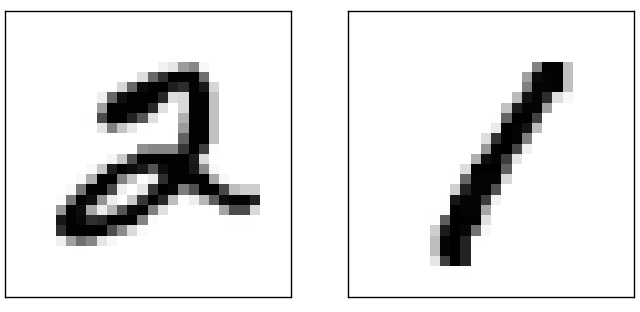
\includegraphics[height=32pt]{mnist_2_and_1}
\end{center}

这提示我们可以用训练数据来计算数字图像的平均暗度,$0, 1, 2,\ldots, 9$。当有一幅
新的图像呈现,我们先计算图像的暗度,然后猜测它接近哪个数字的平均暗度。这是一
个简单的程序,而且容易编写代码,所以我不会在这里把它们都写出来 —— 如果你有兴趣,
代码在
\href{https://github.com/mnielsen/neural-networks-and-deep-learning/blob/master/src/mnist_average_darkness.py}{GitHub
  仓库}里。但是它和随机地猜测相比有了很大的改进,能取得 $10,000$ 测试图像中
$2,225$ 的精确度,即 $22.25\%$。

找到其它能使精确度达到 $20\%$ 到 $50\%$ 之间的办法也不难。如果你更努力些能超过
$50\%$。但要获得更高的精确度,采用已经被认可的机器学习算法是很有帮助的。让我们尝
试使用其中最著名的算法之一,\emph{支持向量机}\index{支持向量机},或 \emph{SVM}\index{SVM}。如果你不熟悉 SVM,
不用担心,我们不需要去理解 SVM 如何工作的细节。我们将使用
\href{http://scikit-learn.org/stable/}{scikit-learn} Python 程序库,它提供了一个
简单的 Python 接口,包装了一个用于 SVM 的快速的,称为
\href{http://www.csie.ntu.edu.tw/~cjlin/libsvm/}{LIBSVM} 的 C 库。

如果我们用默认设置运行 scikit-learn 的 SVM 分类器,那么它能从 $10,000$ 测试图像
中准确分类 $9,435$。(代码可以从%
  \href{https://github.com/mnielsen/neural-networks-and-deep-learning/blob/master/src/mnist_svm.py}{
    这里}取得)。那是一个很大的改善,远远好于我们幼稚的基于暗度的图像分类方法。
确实,这意味着 SVM 表现得几乎和神经网络一样好,只是差了一点而已。在后面章节中我
们会介绍新的技术,让我们能够改进我们的神经网络使得它们表现得比 SVM 更好。

这不是故事的结局,然而,$10,000$ 中 $9,435$ 的结果是 scikit-learn 针对 SVM 默认
的设置。SVM 有很多可调参数,查找到可以改善默认情况下的性能的参数是可能的。我不会
明确地做这些查找,如果你想知道更多,可以参考这份
\href{http://peekaboo-vision.blogspot.ca/}{Andreas Mueller} 的%
\href{http://peekaboo-vision.blogspot.de/2010/09/mnist-for-ever.html}{博客}。
Mueller 展示了通过一些优化 SVM 参数的工作,有可能把性能提高到 98.5\% 的精确度。
换句话说,一个调整好的 SVM,70 次里只会识别错一次数字。那已经非常好了!神经网络
能做得更好吗?

事实上,它们可以。目前,精心设计的神经网络胜过任何其它解决 MNIST 的技术,包括
SVM。现在(2013)的纪录是从 $10,000$ 图像中正确分类 $9,979$ 个。这是由
\href{http://www.cs.nyu.edu/~wanli/}{Li Wan},
\href{http://www.matthewzeiler.com/}{Matthew Zeiler},Sixin Zhang,
\href{http://yann.lecun.com/}{Yann LeCun},和
\href{http://cs.nyu.edu/~fergus/pmwiki/pmwiki.php}{Rob Fergus} 完成的。我们将在
这本书后面看到它们用的大部分技术。那个层次的性能接近于人类,而且可以说更好,因为
相当多的 MNIST 图像甚至对人类来说都很难有信心识别,例如:
\begin{center}
  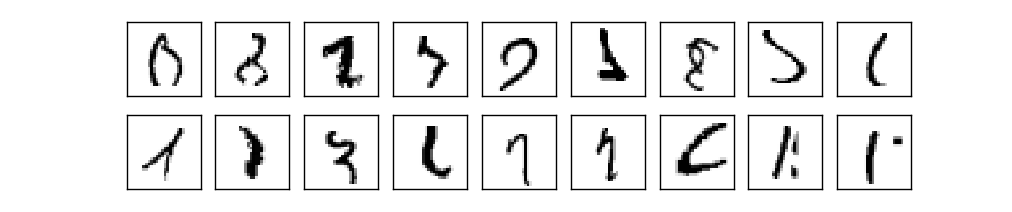
\includegraphics[height=64pt]{mnist_really_bad_images}
\end{center}

我相信你会同意那些数字很难辨认!考虑到 MNIST 数据集中这样的图像,神经网络能准确
识别 $10,000$ 幅测试图像中除了 $21$ 幅之外的其它所有图像,这表现得相当卓越。通常,
当编程时我们相信解决一个类似识别 MNIST 数字的问题需要一个复杂的算法。但是即使是
刚才提到的 Wan 等人的论文中用的神经网络,只涉及到相当简单的算法、和我们在这一章
中已经看到的算法的变化形式。所有的复杂性自动从训练数据学习。在某种意义上,我们的
结果和那些在更深奥的论文中都有的寓意是,对有些问题:

\begin{center}
  复杂的算法 $\leq$ 简单的学习算法 + 好的训练数据
\end{center}

\section{迈向深度学习}

虽然我们的神经网络给出了令人印象深刻的表现,但这样的表现带有几分神秘。网络中的权
重和偏差是被自动发现的。这意味着我们不能立即解释网络怎么做的、做了什么。我们能否
找到一些方法来理解我们的网络通过什么原理分类手写数字?并且,在知道了这些原理后,
我们能做得更好吗?

为了让这些问题更具体,我们假设数十年后神经网络引发了人工智能(AI)。到那个时候,
我们能明白这种智能网络的工作机制吗?或许,因为有着自动学习得到的权重和偏差,这些
是我们无法理解的,这样的神经网络对我们来说是不透明的。在人工智能的早期研究阶段,
人们希望在构建人工智能的努力过程中,也同时能够帮助我们理解智能背后的机制,以及人
类大脑的运转方式。但结果可能是我们既不能够理解大脑的机制,也不能够理解人工智能的
机制。

为解决这些问题,让我们重新思考一下我在本章开始时所给的人工神经元的解释,作为一种
衡量证据的方法。假设我们要确定一幅图像是否显示有人脸:

\begin{center}
\begin{minipage}{0.26\textwidth}
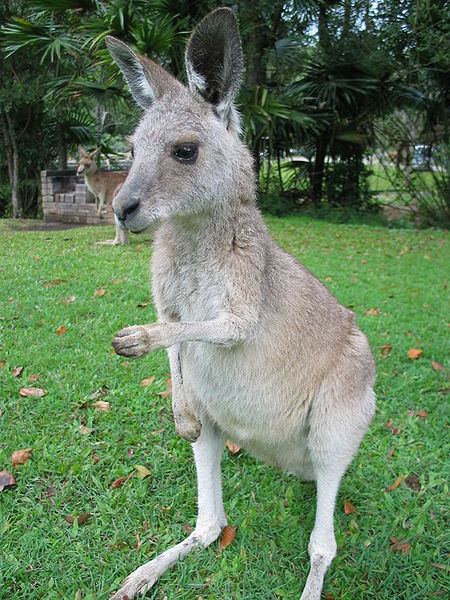
\includegraphics[width=\textwidth]{images/Kangaroo_ST_03}
\end{minipage}
\begin{minipage}{0.24\textwidth}
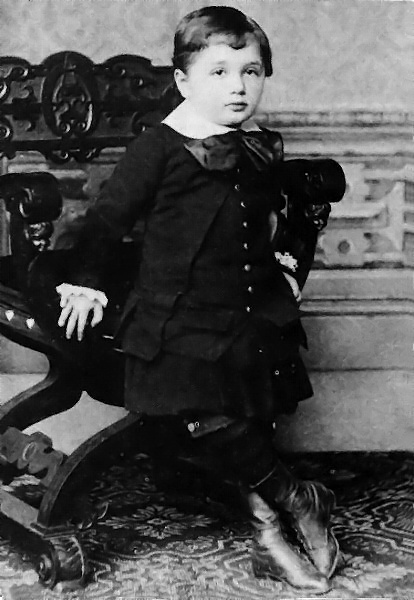
\includegraphics[width=\textwidth]{images/Albert_Einstein_at_the_age_of_three_(1882)}
\end{minipage}
\begin{minipage}{0.4\textwidth}  
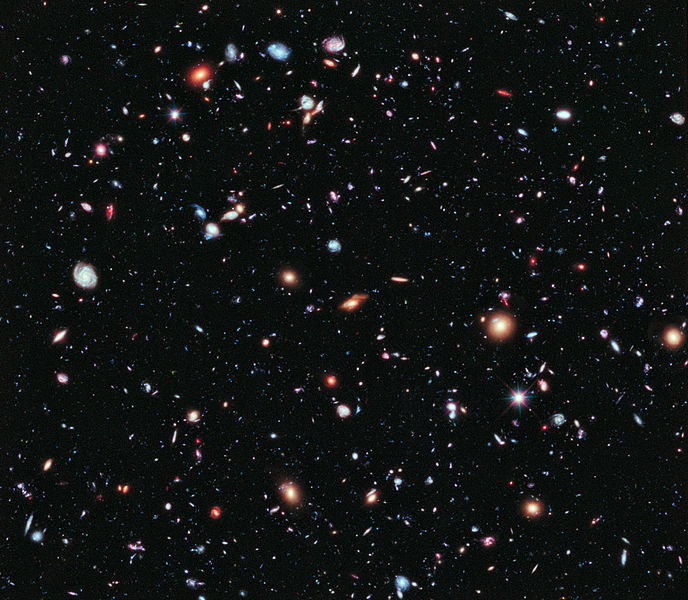
\includegraphics[width=\textwidth]{images/The_Hubble_eXtreme_Deep_Field}
\end{minipage}
\\
\begin{minipage}{0.9\textwidth}
  \footnotesize 照片来
  源:
  \href{http://commons.wikimedia.org/wiki/File:Kangaroo_ST_03.JPG}{1}. \href{http://commons.wikimedia.org/wiki/User:ST}{Ester
    Inbar}. \href{http://commons.wikimedia.org/wiki/File:Albert_Einstein_at_the_age_of_three_(1882).jpg}{2}. Unknown. \href{http://commons.wikimedia.org/wiki/File:The_Hubble_eXtreme_Deep_Field.jpg}{3}. NASA,
  ESA, G. Illingworth, D. Magee, and P. Oesch (University of California, Santa
  Cruz), R. Bouwens (Leiden University), and the HUDF09 Team. 点击序号查看跟多细
  节。
\end{minipage}
\end{center}

我们可以用解决手写识别问题的相同方式来攻克这个问题 —— 网络的输入是图像中的像素,
网络的输出是一个单个的神经元用于表明``是的,这是一张脸''或``不,这不是一张脸''。

假设我们就采取了这个方法,但接下来我们先不去使用一个学习算法。而是去尝试亲手设计
一个网络,并为它选择合适的权重和偏差。我们要怎样做呢?暂时先忘掉神经网络,我们受
到启发的一个想法是将这个问题分解成子问题:图像的左上角有一个眼睛吗?右上角有一个
眼睛吗?中间有一个鼻子吗?下面中央有一个嘴吗?上面有头发吗?诸如此类。

如果一些问题的回答是``是'',或者甚至仅仅是``可能是'',那么我们可以作出结论这个图
像可能是一张脸。相反地,如果大多数这些问题的答案是``不是'',那么这张图像可能不是
一张脸。

当然,这仅仅是一个粗略的想法,而且它存在许多缺陷。也许有个人是秃头,没有头发。也
许我们仅仅能看到脸的部分,或者这张脸是有角度的,因此一些面部特征是模糊的。不过这
个想法表明了如果我们能够使用神经网络来解决这些子问题,那么我们也许可以通过将这些
解决子问题的网络结合起来,构成一个人脸检测的神经网络。下图是一个可能的结构,其中
的方框表示子网络。注意,这不是一个人脸检测问题的现实的解决方法,而是为了帮助我们
构建起网络如何运转的直观感受。下图是这个网络的结构:

% tikz14.png
\begin{center}
  \begin{tikzpicture}
    [question/.style={rectangle,draw,minimum width=5cm,minimum height=1.5cm}]

    \foreach \y in {0,...,9}
      \node(i\y) at (-5, -3.6 + \y / 1.25) [circle,draw,minimum size=6mm] {};

    \node(q0) [question] {
      \footnotesize 中间有一个鼻子吗?
    };
    \node(q1) [question,above=5mm of q0] {
      \footnotesize 右上角有一个眼睛吗?
    };
    \node(q2) [question,above=5mm of q1] {
      \footnotesize 左上角有一个眼睛吗?
    };    
    \node(q3) [question,below=5mm of q0] {
      \footnotesize 下面有一个嘴吗?
    };
    \node(q4) [question,below=5mm of q3] {
      \footnotesize 上面有头发吗?
    };

    \node(n) [circle,draw,right=2cm of q0,minimum size=6mm] {};
    \node(o) [right=of n] {
      \footnotesize 这是张人脸吗?
    };
    
    \node(text) [above=5mm of i9] {
      \begin{tabular}{c}
        {\footnotesize input layer}\\
        {\footnotesize (image pixels)}\\
      \end{tabular}
    };

    % connections:
    \foreach \x in {0,...,9}
      \foreach \y in {0,...,4}
        \draw[->] (i\x) to (q\y.west);

    \foreach \x in {0,...,4}
      \draw[->] (q\x.east) to (n);
      
    \draw[->] (n) to (o);

  \end{tikzpicture}
\end{center}

子网络也可以被继续分解,这看上去很合理。假设我们考虑这个问题:``左上角有一个眼睛
吗?''。 这个问题可以被分解成这些子问题:``有一个眉毛吗?'',``有睫毛吗?'',
``有虹膜吗?'',等等。当然这些问题也应该包含关于位置的信息 —— 诸如``在左上角有眉
毛,上面有虹膜吗?'' —— 但是让我们先保持简单。回答问题``左上角有一个眼睛吗?''的
网络能够被分解成:

% tikz15.png
\begin{center}
  \begin{tikzpicture}
    [subquestion/.style={rectangle,draw,minimum width=4cm,minimum height=1.5cm},
     mainquestion/.style={rectangle,draw,minimum width=5cm,minimum height=1.5cm}]

    \node(t1) [subquestion] {
      \footnotesize 有一个眉毛吗?
    };
    \node(t2) [subquestion,above=5mm of t1] {
      \footnotesize 有睫毛吗?
    };
    \node(t3) [subquestion,below=5mm of t1] {
      \footnotesize 有一个虹膜吗?
    };
    \node(equal) [left=5mm of t1] {$=$};
    \node(t4) [mainquestion,left=5mm of equal] {
      \footnotesize 左上角有一个眼睛吗?
    };

    \node(n) [circle,draw,right=of t1,minimum size=6mm] {};
    \node(o) [right=of n] {};

    \draw[->] (t1.east) to (n);
    \draw[->] (t2.east) to (n);
    \draw[->] (t3.east) to (n);
    \draw[->] (n) to (o);

  \end{tikzpicture}
\end{center}

这些子问题也同样可以继续被分解,并通过多个网络层传递得越来越远。最终,我们的子网
络可以回答那些只包含若干个像素点的简单问题。举例来说,这些简单的问题可能是询问图
像中的几个像素是否构成非常简单的形状。这些问题就可以被那些与图像中原始像素点相连
的单个神经元所回答。

最终的结果是,我们设计出了一个网络,它将一个非常复杂的问题 —— 这张图像是否有一张
人脸 —— 分解成在单像素层面上就可回答的非常简单的问题。它通过一系列多层结构来完成,
在前面的网络层,它回答关于输入图像非常简单明确的问题,在后面的网络层,它建立了一
个更加复杂和抽象的层级结构。包含这种多层结构 —— 两层或更多隐藏层 —— 的网络被称为%
\emph{深度神经网络}\index{深度神经网络}。

当然,我没有提到如何去递归地分解成子网络。手工设计网络中的权重和偏差无疑是不切实
际的。取而代之的是,我们希望使用学习算法来让网络能够自动从训练数据中学习权重和偏
差 —— 这样,形成一个概念的层次结构。80 年代和 90 年代的研究人员尝试了使用随机梯
度下降和反向传播来训练深度网络。不幸的是,除了一些特殊的结构,他们并没有取得很好
的效果。虽然网络能够学习,但是学习速度非常缓慢,不适合在实际中使用。

自 2006 年以来,人们已经开发了一系列技术使深度神经网络能够学习。这些深度学习技术
基于随机梯度下降和反向传播,并引进了新的想法。这些技术已经使更深(更大)的网络能
够被训练 —— 现在训练一个有 5 到 10 层隐藏层的网络都是很常见的。而且事实证明,在
许多问题上,它们比那些浅层神经网络,例如仅有一个隐藏层的网络,表现的更加出色。当
然,原因是深度网络能够构建起一个复杂的概念的层次结构。这有点像传统编程语言使用模
块化的设计和抽象的思想来创建复杂的计算机程序。将深度网络与浅层网络进行对比,有点
像将一个能够进行函数调用的程序语言与一个不能进行函数调用的精简语言进行对比。抽象
在神经网络中的形式和传统的编程方式相比不同,但它同样重要。
